\chapter{Topological stabilizer codes}
\label{Chap:TpologicalCodes}
Protecting quantum information from decoherence is of prime importance to realize quantum information processing.
Several approaches have been proposed toward reliable quantum information processing, ranging from passive to active protections, such as decoherence-free subspaces
\cite{DFS}, dynamical decoupling \cite{DD}, and quantum error correction \cite{Shor95}.
Among these, the most comprehensive approach is fault-tolerant quantum computation based on quantum error correction \cite{DiViShor}.
Quantum fault-tolerance theory ensures scalable quantum computation with noisy quantum devices as long as the error probability of such devices is smaller than a threshold value (see Appendix~\ref{Ap:FT_syndrome_meas}). 
The first threshold values were obtained, at almost the same time (1996), independently by Aharonov {\it et al.}, who used a polynomial code of distance five \cite{Aharonov97,Aharonov08}; Knill {\it et al.}, who used the Steane seven-qubit code \cite{Knill98a,Knill98b}; and Kitaev, who used toric (surface) codes \cite{Kitaev97}.
All of these studies were based on a concatenated quantum computation and achieved similar threshold values $\sim 10^{-6}$. 
Since then, fault-tolerant quantum computing has been studied as one of the most important issues in quantum information science.
In 2005, Knill proposed a novel scheme based on the $C_4/C_6$ error-detecting code, namely the Fibonacci scheme \cite{KnillNature}, and achieved a considerably higher threshold, a few \%. 
Recently, Fujii {\it et al.} have further improved this approach by making use of measurement-based quantum computation (MBQC) \cite{RaussendorfAnn,RaussendorfNJP} on logical cluster states, which gives the highest threshold value so far, $\sim 5\%$ \cite{FYCluster,FYClusterTopo}.

All these approaches rely on the availability of two-qubit gates between arbitrarily separated qubits.
However, all physically available interactions are local in space. 
Moreover, if we consider manufacturing convenience and the selective addressability of individual qubits, 2D nearest-neighbor architectures are necessary.
It was thought that, if we restrict the two-qubit gates to nearest-neighbor ones in 2D, then the threshold value would decrease significantly \cite{Svore}.
The situation changed completely by the proposal made by Raussendorf {\it et al.}, i.e., topologically protected quantum computation~\cite{RaussendorfPRL,RaussendorfNJP,RaussendorfAnn}. 
They utilized a surface code, a kind of topological quantum code, originally proposed by Kitaev as a toric code on a torus~\cite{Kitaev} and investigated by Dennis {\it et al.} in detail~\cite{Dennis}.
All the stabilizer generators of the surface code are spatially local, as will be seen later, and hence syndrome measurements are done by using nearest-neighbor two-qubit gates.
More importantly, Raussendorf {\it et al.} developed a novel way to implement a fault-tolerant logical gate operation by braiding defects on the surface, which can be done by using only single-qubit measurements and nearest-neighbor two-qubit gates.
Nevertheless, its threshold value is very high $\sim 1\%$~\cite{RaussendorfPRL,RaussendorfNJP,RaussendorfAnn,WangFowler}.
Based on these analyses, physical implementations and quantum architecture designs have recently been suggested~\cite{VanMeter,LiBenjamin,FTProb,Jones12,FujiiDis,Benjamin1,Benjamin2,Fowler1,Fowler2}, which clarifies the experimental requirements for building a fault-tolerant quantum computer.
On the other side, extensive experimental resources have been used to achieve these requirements, and very encouraging results have already been obtained in several experiments 
in superconducting systems \cite{Chow12IBM,IBM13,UCSB14,IBM14}.

Another important motivation for studying topological quantum codes are their connection with topologically ordered systems in condensed matter physics~\cite{Kitaev}.
Topological stabilizer codes, whose stabilizer generators are local and translation invariant, provide toy models for topologically ordered systems.
Using quantum coding theory with a geometrical constraint such as locality and translation invariance, we can understand the nature of topologically ordered condensed matter systems.
One of the most important issues in this direction is to answer whether or not thermally stable topological order exists in three or lower dimensions~\cite{BravyiTerhal,BeniThermal3D}.

When we consider the decoding problems of topological quantum codes, we encounter classical statistical physics~\cite{Dennis}.
Specifically, the posterior probabilities for the error correction correspond to partition functions of classical spin glass models~\cite{Dennis}, such as the random-bond Ising model.
If the corresponding random-bond Ising model lies inside a ferromagnetic phase, the error correction on a surface code succeeds, and the logical error probability decreases exponentially.

In this chapter, we introduce a representative example of the topological stabilizer codes\index{topological stabilizer code}, the surface codes. 
Before that, we also briefly review the ${\bf Z}_2$ chain complex, which is a useful tool to define the surface codes. 
We also apply it to a classical repetition code as an exercise.
After introducing the surface codes, we explain how topological error correction is performed.
We also mention the relation between topological error correction and the classical spin glass model.
Another example of topological stabilizer codes, the topological color codes, is also presented.
Finally, we explain the connection between topological stabilizer codes and topologically ordered systems studied in condensed matter physics.




\section{${\bf Z}_2$ chain complex}
\label{sec:chain_complex}
Before defining the surface codes, we introduce a mathematical tool, the $\mathbf{Z}_2$ chain complex\index{$\mathbf{Z}_2$ chain complex}, which is useful for describing the surface codes. 

Consider a surface $G=(V,E,F)$ that consists of the vertices $V=\{v_k\}$, edges $E=\{e_l\}$, and faces $F=\{f_m\}$.
(Here we consider a graph $G=(V,E)$ embedded on a 2D manifold, the {\it surface}, on which the faces $F$ are defined.)
We define a vector space $C_0$ over $\mathbf{Z}_2$, using each vertex $v_k \in V$ as a basis $B(C_0)=\{ v_k\}$.
A vector in $C_0$
\begin{eqnarray}
c_0 &=& \sum _k z_k v_k, 
\end{eqnarray}
where $z_k =\{ 0, 1\}$, is referred to as a 0-chain.
The vector space $C_0$ is an Abelian group under component-wise addition modulo 2.
Similarly, we can define the Abelian groups $C_1$ and $C_2$ using the edges $E=\{e_l\}$ and faces $F=\{ f_m \}$ as base vectors $B(C_1)=\{ e_l\}$ and $B(C_2)=\{ f_m\}$, respectively.
The elements
\begin{eqnarray}
c_1 &=& \sum _l z_l e_l, \;\;\;
\\
c_2 &=& \sum _m z_m f_m, \;\;\;
\end{eqnarray}
where $z_l, z_m=\{ 0,1\}$, are called the 1-chain and 2-chain, respectively.
With a mild abuse of the notation, a set of $i$-dimensional elements (i.e., vertices, edges, and faces) is also specified by a $i$-chain $c_i \in C_i$ as a set of elements having $z_j=1$.

We can define a homomorphism $\partial_i : C_i \rightarrow C_{i-1}$ such that 
\begin{eqnarray}
\partial _i \circ \partial _{i-1}=0.
\label{eq:boundary_op}
\end{eqnarray} 
Specifically, $\partial _i c_i $ is defined as an $(i-1)$-chain that is the boundary of $c_i$. 
For example, $\partial e_l$ is a 1-chain for which $z_k=1$ if and only if (iff) $v_k$ is an endpoint of $e_l$.
Thus, the homomorphism $\partial _i$ is called a boundary operator.
When there is no risk for confusion, we will denote $\partial _i$ simply by $\partial$.
A chain $c_i$ is called a cycle, if it is in a kernel of the boundary operator $\partial _i$, i.e., $\partial c_i=0$.
For example, the boundary $\partial_2 f_m$ of a face $f_m$ is a cycle, because $\partial _2 \circ \partial _1 =0$. 
Such a sequence of Abelian groups $C_i$, connected by the boundary operators $\partial _i$ with $\partial _i \circ \partial _{i-1}=0$, is called a $\mathbf{Z}_2$ chain complex.
We define a trivial $i$-cycle $c_i$ if there exists an $(i+1)$-chain such that $c_i = \partial c_{i+1}$, i.e., $c_i \in {\rm Img} (\partial _{i+1})$.
By regarding the trivial cycles\index{trivial cycle} as generators of the continuous deformation, we may define an equivalent class having the same topology.
More precisely, a homology group $h_i$ is defined as a quotient group\index{quotient group} formed by the cycles and the trivial cycles:
\begin{eqnarray}
h_i = \ker (\partial _i) / {\rm Img} (\partial _{i+1}).
\end{eqnarray}
An element of the quotient group $h_i$ is called a homology class\index{homology class}.
If two $i$-chains $c_i$ and $c'_i$ belong to the same homology class, there exists an $(i+1)$-chain $c_{i+1}$ such that $c_i = c'_i + \partial c_{i+1}$.
Two such $i$-chains $c_i$ and $c'_i$ are said to be homologically equivalent.

We also define the dual surface $\bar G=(\bar V,\bar E,\bar F)$, where we identify the elements of the dual and original (primal) lattices such that $\bar V=F$, $\bar E=E$ and $\bar F=V$.
Specifically, the dual lattice is constructed such that the two vertices $\bar v, {\bar v}' \in \bar V$ are connected by an edge $\bar e$, if the corresponding two faces $f$ and $f'$ share the same edge $e$.
We can also define a $\mathbf{Z}_2$ chain complex on $\bar G$ using the dual bases $\bar B(C_i)$, a dual $i$-chain $\bar c_i \in \bar C_i$ and a boundary operator 
$\bar \partial _i: \bar C_i \rightarrow \bar C_{i-1}$.
When there is no risk of confusion, $\bar \partial _i$ will be denoted by $\partial$.
 
In the construction of the surface codes, a qubit is defined on each edge $e_l \in E$ of the surface $G$ (or equivalently each dual edge $\bar e_l$ of the dual surface $\bar G$).
The Pauli product is defined using a 1-chain $c_1 = \sum _l z_l e_l$ (or dual 1-chain $\bar c_1$) such that
\begin{eqnarray}
W(c_1) = \prod _{l} W_l^{z_l},
\end{eqnarray}
where $W_l \in \{X_l , Y_l,Z_l \}$ is a Pauli operator acting on the qubit on edge $e_l$.
Specifically, we have 
\begin{eqnarray}
W(c_1)W(c'_1)=W(c_1 + c'_1).
\end{eqnarray}
Consider the two operators $X(c_1)$ and $Z(c'_1)$, defined by the two 1-chains $c_1$ and $c'_1$, respectively.
The commutability of these two operators is determined by the inner product of the two chains (vectors) $c_1\cdot c'_1 \equiv \sum _{l}z_l z'_l$, where the addition is taken modulo 2:
\begin{eqnarray}
c_1\cdot c'_1 &=&0, \;\; {\rm iff} \;\; X(c_1)Z(c'_1)=Z(c'_1)X(c_1) \;\; {\rm (commute)},
\\
c_1\cdot c'_1&=&1, \;\; {\rm iff} \;\; X(c_1)Z(c'_1)=-Z(c'_1)X(c_1) \;\; {\rm (anticommute)}.
\end{eqnarray}

Let $M(\partial _i)$ be a matrix representation of $\partial _i$ with respect to the basis vectors $B(C_i)$ and $B(C_{i-1})$.
We have
\begin{eqnarray}
\bigl(M(\partial _i) c_i \bigr) \cdot c_{i-1} =  c_i \cdot \bigl( M(\partial _i)^{T}  c_{i-1} \bigr).
\label{eq:adjoint}
\end{eqnarray}
By identifying the primal and dual bases $B(C_0)=\bar B(C_2)$, $B(C_1)=\bar B(C_1)$, and $B(C_2)=\bar B(C_0)$, the duality relation between primal and dual lattices can be expressed by
\begin{eqnarray}
M(\partial _1) = M(\bar \partial _2)^{T},
\;\;\;
M(\partial _2) = M(\bar \partial _1)^{T},
\label{eq:dual_rep}
\end{eqnarray}
where $[\cdot]^{T}$ indicates the matrix transpose.

Using Eq.\ (\ref{eq:boundary_op}) $\partial _1 \circ \partial _2=0$, we obtain $ M(\bar \partial _2)^{T} M(\partial _2)=0$.
Thus, for any primal and dual 2-chains, $c_2$ and $\bar c_2$, we have 
\begin{eqnarray}
\bar \partial \bar c_2 \cdot \partial c_2=0,
\label{eq:commutability}
\end{eqnarray}
i.e., $X(\partial c_2)$ and $Z(\bar \partial \bar c_2)$ always commute.
This property is useful to construct a stabilizer group, because stabilizer generators have to commute with each other.
Using Eqs.\ (\ref{eq:adjoint}) and (\ref{eq:dual_rep}), we also have
\begin{eqnarray}
c_1 \cdot \bar \partial _{2} \bar c_2 = \partial c_1 \cdot \bar c_2.
\label{eq:comm_rep}
\end{eqnarray}



\section{A bit-flip code: exercise}
\label{sec:bit-flip}
\begin{figure}[t]
\centering
%\sidecaption
% Use the relevant command for your figure-insertion program
% to insert the figure file.
% For example, with the option graphics use
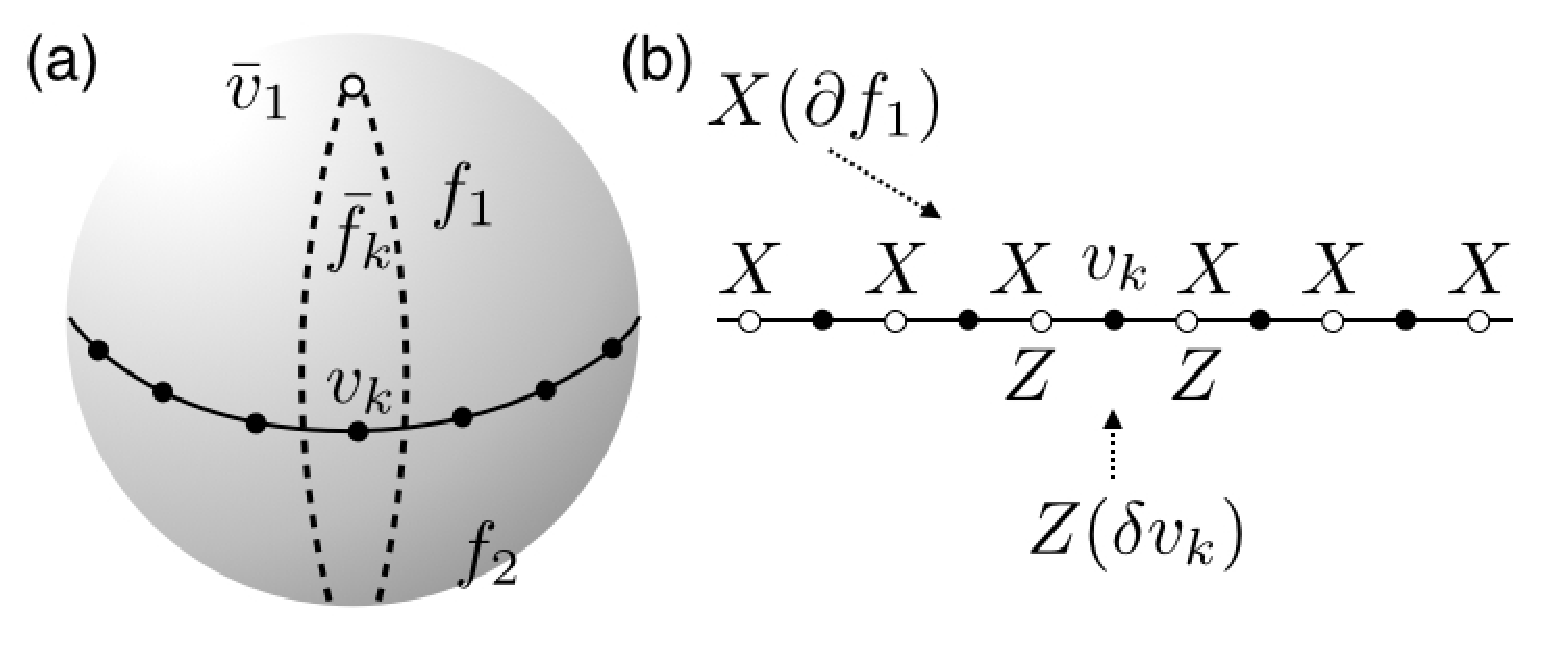
\includegraphics[width=130mm]{fig54.eps}
%
% If not, use
%\picplace{5cm}{2cm} % Give the correct figure height and width in cm
%
\caption{(a) A regular polygon embedded on a sphere. (b) A stabilizer operator defined as $A_k=Z(\partial \bar f_k)=\prod _{\delta v_k} Z_k$. 
The logical $X$ operator is given by $L_X=X(\partial f_1)$. Because primal and dual 1-chains share an even number of qubits, $L_X$ and $A_k$ commute with each other. }
\label{fig54}       % Give a unique label
\end{figure}
%%%%%%%%%%%%%%%%%%%%%%%%%%%
%%%%%%%%%%%%%%%%%%%%%%%%%%%
%%%%%%%%%%%%%%%%%%%%%%%%%%%
As an exercise, we define a bit-flip code (classical repetition code) using the $\mathbf{Z}_2$ chain complex.
(Readers who are familiar with this topic may skip this section.)
Consider a regular polygon $G(V,E,F)$ on a sphere consisting of $n=|E|$ edges and two faces $F=\{ f_1 , f_2\}$ (corresponding to the top and bottom hemispheres) as shown in Fig.~\ref{fig54}.
The number of qubits is $n$.

We define a stabilizer generator for each dual face $\bar f _k= v_k$ as follows:
\begin{eqnarray}
A_{k}=Z( \partial \bar f_k)= \prod _{e_l \in \delta v_k} Z_l,
\end{eqnarray}
where, for convenience, $\delta v_k \equiv \partial \bar f $ is defined as a set of edges that are incident to the vertex $v_k$.
(Note that both the dual and primal objects are identified.)

Because $ \prod _{v_k \in V} A_k = I$, there are $n-1$ independent stabilizer generators.
The dimension of the stabilizer subspace is two.
The code subspace is described by a one-cycle $c_1= \partial f_1=\partial f_2$ surrounding the sphere. 
We define the logical $X$ operator
\begin{eqnarray}
L_X=X(\partial f_1)= X(c_1).
\end{eqnarray}
Note that $L_X=X(\partial f_1)$ and $A_{k}=Z( \partial \bar f_k)$ commute, due to Eq.\ (\ref{eq:commutability}).
The logical Pauli $Z$ operator, which commutes with $\{ A_k\}$ and anticommutes with $L_X$, is defined as $L_Z= Z_l$.
(We may choose any of the $Z_l$s on the edge $e_l$, because they act equivalently on the code space.)
The code is a bit-flip code, which protects quantum information against bit flip errors.

\begin{figure}[t]
\centering
%\sidecaption
% Use the relevant command for your figure-insertion program
% to insert the figure file.
% For example, with the option graphics use
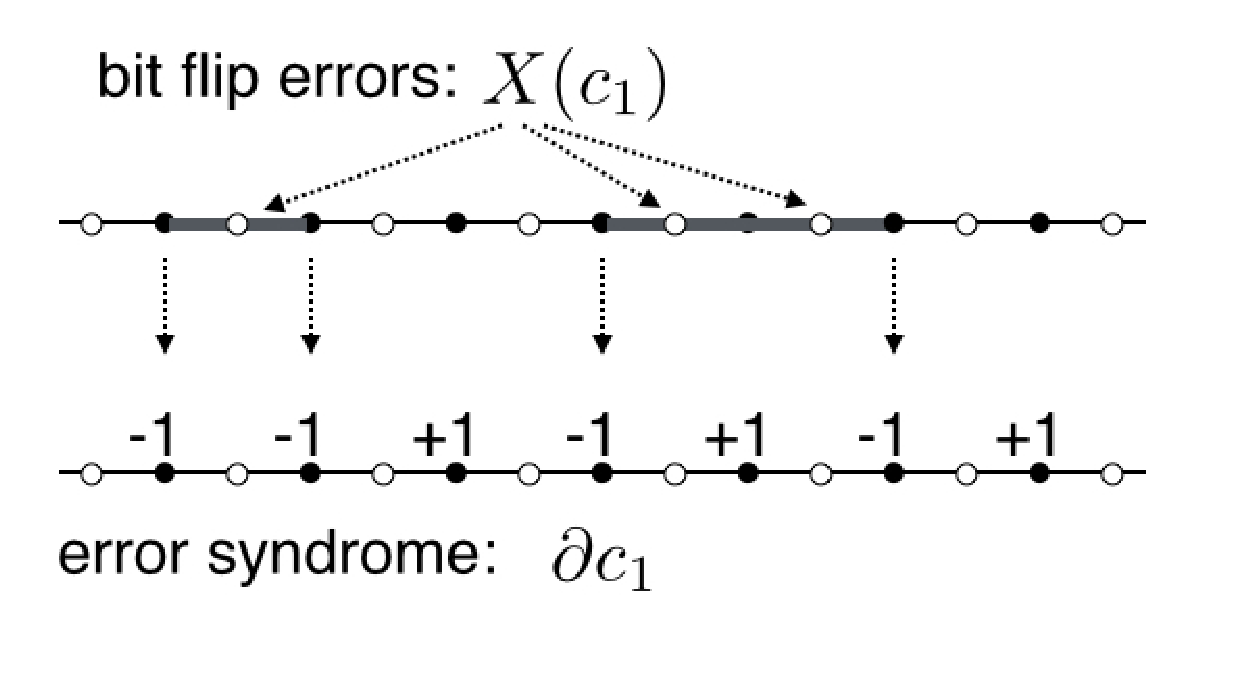
\includegraphics[width=110mm]{fig55.eps}
%
% If not, use
%\picplace{5cm}{2cm} % Give the correct figure height and width in cm
%
\caption{An $X$ error chain $X(c_1)$ and the corresponding error syndrome $\partial c_1$.
The eigenvalue of the stabilizer generator becomes $-1$ on vertices in $\partial c_1$.}
\label{fig55}       % Give a unique label
\end{figure}
%%%%%%%%%%%%%%%%%%%%%%%%%%%
%%%%%%%%%%%%%%%%%%%%%%%%%%%
%%%%%%%%%%%%%%%%%%%%%%%%%%%
A string of bit errors $X(c_1)$ is defined using a 1-chain $c_1$, which we call an error chain.
The error is detected by measuring the eigenvalues of the stabilizer generators $A_k=Z(\delta v_k)$, i.e., through syndrome measurements.
From Eq.\ (\ref{eq:comm_rep}), we have $c_1 \cdot \delta v_k = \partial c_1 \cdot v_k$.
Thus, $X(c_1)$ anticommutes with the stabilizer generator $A_k$ if $\partial c_1 \cdot v_k =1$. 
Hence, $X(c_1)$ anticommutes with $A_k$ on the vertex $v_k$ that is a boundary $v_ k \in \partial c_1$ of the error chain $c_1$.
The eigenvalue of the stabilizer generator becomes -1.
Error correction is the task of finding a recovery chain $c'_1$ such that $\partial (c_1 + c'_1)=0$.
In the case of the bit-flip code, there are only two possibilities $c_1+c'_1=0$ or $c_1+c'_1=\partial f_1$.
In the former case, error correction succeeds, while the latter case results in a logical error $L_X$.

The bit-flip code cannot protect quantum information against phase errors. 
A natural extension of the classical repetition code to handle both bit and phase errors is the surface codes introduced in the next section.

\section{Definition of surface codes}
\subsection{Surface code on a torus: toric code}
\begin{figure}[t]
\centering
%\sidecaption
% Use the relevant command for your figure-insertion program
% to insert the figure file.
% For example, with the option graphics use
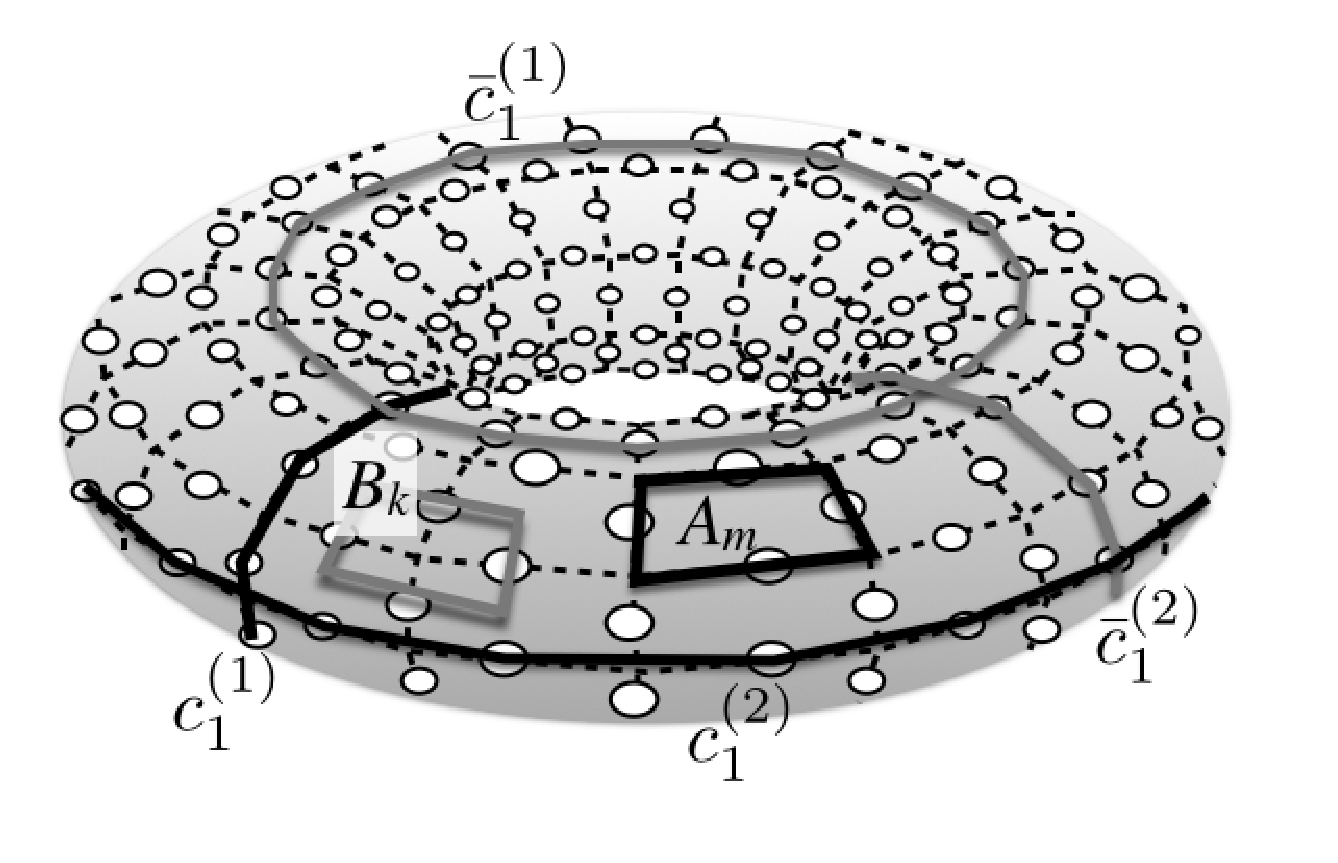
\includegraphics[width=100mm]{fig56.eps}
%
% If not, use
%\picplace{5cm}{2cm} % Give the correct figure height and width in cm
%
\caption{A square lattice on a torus with a periodic boundary condition. 
The $Z$ and $X$ stabilizer generators are defined by being associated with each face and vertex (dual face). 
The logical $Z$ and $X$ operators are defined by non-trivial cycles.}
\label{fig56}       % Give a unique label
\end{figure}
%%%%%%%%%%%%%%%%%%%%%%%%%%%
%%%%%%%%%%%%%%%%%%%%%%%%%%%
%%%%%%%%%%%%%%%%%%%%%%%%%%%
Now we are ready to define the surface code.
Let us consider a square lattice $G=(V,E,F)$ on a torus with a periodic boundary condition as shown in Fig.~\ref{fig56}.
A dual square lattice $\bar G=(\bar V, \bar E, \bar F)$ is also defined on the torus.
We define stabilizer generators of the $Z$- and $X$-types for each face $f_m$ and vertex $v_k$ as follows:
\begin{eqnarray}
A_m=Z(\partial f_m), \;\;\;  B_k=X(\delta v_k)=X(\partial \bar f_k).
\end{eqnarray}
Because $\partial f_m \cdot \partial \bar f_k =0$ from Eq.\ (\ref{eq:commutability}), $A_m$ and $B_k$ commute.
The stabilizer generators $A_m$ and $B_k$ are called plaquette and star operators \index{plaquette and star operators}, respectively.
By the definition of the stabilizer code, the code state $|\Psi\rangle$ satisfies 
\begin{eqnarray}
A_m |\Psi \rangle = |\Psi \rangle , \;\;\; B_k |\Psi \rangle = |\Psi \rangle,
\end{eqnarray}
for all $f_m \in F$ and $v_k \in V$.

%%%%%%
If two 1-chains, $c_1$ and $c'_1$, are homologically equivalent, the actions of $Z(c_1)$ and $Z(c'_1)$ on the code state are the same, because there exists a 2-chain $c_2$ such that 
\begin{eqnarray}
Z(c'_1)=Z(c_1)Z(\partial c_2)=Z(c_1) \left(\prod _{f_m \in c_2}A_m\right).
\label{eq:homo_eq}
\end{eqnarray}
We will denote this simply by $Z(c'_1) \sim Z(c_1)$.
This is also the case for homologically equivalent dual 1-chains, $\bar c_1$ and $\bar c'_1$, and the actions of $X(\bar c_1)$ and $X(\bar c'_1)$ on the code state.
Hence, the homology classes, which are equivalent classes over trivial cycles, of the primal and dual 1-chains correspond to the actions of $Z$- and $X$-type operators on the code state, because their actions are equal up to stabilizer operators.
%%%%%%

Let us define the logical operators $Z(c_1)$ and $X(\bar c_1)$.
The logical operators have to commute with all stabilizer generators and also be independent of them.
The former condition implies that $\partial c_1 =0$ and $\partial \bar c_1=0$ from Eq.\ (\ref{eq:comm_rep}).
This is because the commutability imposes that $c_1 \cdot \delta v_k = \partial c_1 \cdot v_k =0$ for all vertices $k$ and 
$\bar c_1 \cdot \partial f_m = \partial \bar c_1 \cdot \bar v_m=0$ for all faces (dual vertices) $m$.
The latter condition implies that $c_1$ and $\bar c_1$ are nontrivial cycles, because for two homologically equivalent cycles $c_1$ and $c'_1$, the actions of $Z(c_1)$ and $Z(c'_1)$ on the code state are the same
as seen in Eq.(\ref{eq:homo_eq}).
We can find two non-trivial cycles, which belong to different homology classes, for each primal and dual 1-chain, as shown in Fig.~\ref{fig56}.
(This is a natural consequence, because the homology group $h_1$ on the torus is $\mathbf{Z}_2 \times \mathbf{Z}_2$.)
Then, we define two pairs of logical Pauli operators
\begin{eqnarray}
\{ L_Z^{(1)}=Z(c_1^{(1)}), L_X^{(1)}=X(\bar c_1^{(1)})\}
\;\; {\rm and} \;\;
\{ L_Z^{(2)}=Z(c_1^{(2)}), L_X^{(2)}=X(\bar c_1^{(2)})\}.
\end{eqnarray}
Note that $L_Z^{(i)}$ and $L_X^{(j)}$ anticommute with each other if $i=j$.
Otherwise, they commute:
\begin{eqnarray}
L_Z^{(i)}L_X^{(j)} = (-1)^{\delta _{ij}} L_X^{(j)}L_Z^{(i)}.
\end{eqnarray}
%where $\delta _{ij}$ is the Kronecker delta.
That is, they satisfy a commutation relation equivalent to that of the Pauli operators for two qubits.
The logical Pauli basis states are defined as follows:
\begin{eqnarray}
L_Z^{(i)} | \Psi _Z (s_1 ,s_2)\rangle &=& (-1)^{s_i}| \Psi _Z (s_1 ,s_2)\rangle ,
\\
L_X^{(i)} | \Psi _X (s_1 ,s_2)\rangle &=& (-1)^{s_i}| \Psi _X (s_1 ,s_2)\rangle .
\end{eqnarray}
The number of stabilizer generators of the $n \times n$ square lattice on the torus is given by 
\begin{eqnarray}
|F|+|\bar F|-2=|F|+|V|-2=2n^2-2,
\end{eqnarray}
where $-2$ comes from the fact that $\prod_{f_m \in F} A_m=I$ and $\prod_{v_k \in V} B_k=I$, and hence there are two non-independent operators.
On the other hand, the number of qubits is given by 
\begin{eqnarray}
|E| = 2 n^2.
\end{eqnarray}
Thus, we have a $2^{|E|-(|F|+|V|-2)}=2^{2}$-dimensional stabilizer subspace.
The above two pairs of logical operators appropriately describe the degrees of freedom in the code space.
The code distance, the minimum weight of the logical operators, is determined by the linear length of the square lattice.
Thus, the surface code on the torus is an $[[n^2,2,n]]$ stabilizer code.


In short, an operator that commutes with the stabilizer generators corresponds to a cycle, i.e., ${\rm ker}(\partial _1)$.
The stabilizer operators correspond to the boundaries of the 2-chains $c_2 \in C_2$.
The logical operators, which commute with and are independent of the stabilizer generators, correspond to the homology class $h_1 = {\rm ker}(\partial _1)/{\rm Img}(\partial_2)$.
We summarize the correspondence between the surface code and the $\mathbf{Z}_2$ chain complex in Tab.~\ref{tab:ChainStabCode}.
\begin{table}[htdp]
\caption{The correspondence between $\mathbf{Z}_2$ chain complex and stabilizer codes.}
\begin{center}
\begin{tabular}{c|c}
\hline
\hline
stabilizer code & chain complex
\\
\hline
$Z$-type stabilizer generator & face $f_m$
\\
\hline
$X$-type stabilizer generator & vertex $v_k$ (dual face $\bar f_k$)
\\
\hline
$Z$- and $X$-type stabilizer operators & boundaries of 2-chains, 
\\
& ${\rm Img}(\partial _2)$ and  ${\rm Img}(\bar{\partial} _2)$
\\
\hline
commutability & cycle conditions: $\partial c_1 =0$ and $\partial \bar c_1=0$
\\
\hline
the operators commuting with stabilizer generators & ${\rm ker} (\partial _1)$ and  ${\rm ker} (\bar{\partial} _1)$
\\
\hline
the logical $Z$ and $X$ operators & nontrivial cycles $c_1$ and $\bar c_1$
\\
 & (homology classes $[c_1] = {\rm ker}(\partial _1) /{\rm Img}(\partial _2)$ 
 \\
 &
 and $[\bar c_1]={\rm ker}(\bar \partial _1) /{\rm Img}(\bar \partial _2)$)

\\
\hline
$Z$ and $X$ errors & 1-chains $c_1$ and $\bar c_1$
\\
\hline
$Z$ and $X$ error syndromes & $\partial c_1$ and $\partial \bar c_1$
\\
\hline \hline
\end{tabular}
\end{center}
\label{tab:ChainStabCode}
\end{table}%




All properties so far hold for a general tilling $G=(V,E,F)$, and hence we can define a surface code on general, e.g., triangular and hexagonal, lattices~\cite{FujiiTokunaga12}.
Moreover, the numbers of edges, faces, and vertices are subject to the Euler characteristic formula 
\begin{eqnarray}
|F|+|V|-|E| = 2- 2 g,
\end{eqnarray}
where $g$ is the genus, the number of ``handles'' of the surface. 
Thus, the dimension of the stabilizer subspace is calculated to be $2^{|E|-(|F|+|V|-2)}=2^{2g}$.
These are the degrees of freedom equivalent to $2g$ qubits in the stabilizer subspace.

Because almost all arguments are made from the operator viewpoint (Heisenberg picture), there is no need to write down $|\Psi_A(s_1,s_2) \rangle$ explicitly.
However, for the readers who worry about such things, we will give an explicit description from the state viewpoint:
\begin{eqnarray}
|\Psi _Z (s_1,s_2)\rangle &=& \mathcal{N}  Z(c_1^{(1)})^{s_1} Z(c_1^{(2)})^{s_2} \left( \prod _{v_k \in V} \frac{I+B_k}{2} \right) |0\rangle ^{\otimes n^2}
\\
|\Psi _X (s_1,s_2)\rangle &=&\mathcal{N}  X(\bar c_1^{(1)})^{s_1} X(\bar c_1^{(2)})^{s_2}\left( \prod _{f_m \in F} \frac{I+A_m}{2} \right) |+\rangle ^{\otimes n^2}
\end{eqnarray}
where $\mathcal{N}$ is a normalization factor.
The code state can be viewed as an equal weight superposition of all cycles belonging to the same homology class.

\subsection{Planar surface code}
\label{subsec:planar}
\begin{figure}[t]
\centering
%\sidecaption
% Use the relevant command for your figure-insertion program
% to insert the figure file.
% For example, with the option graphics use
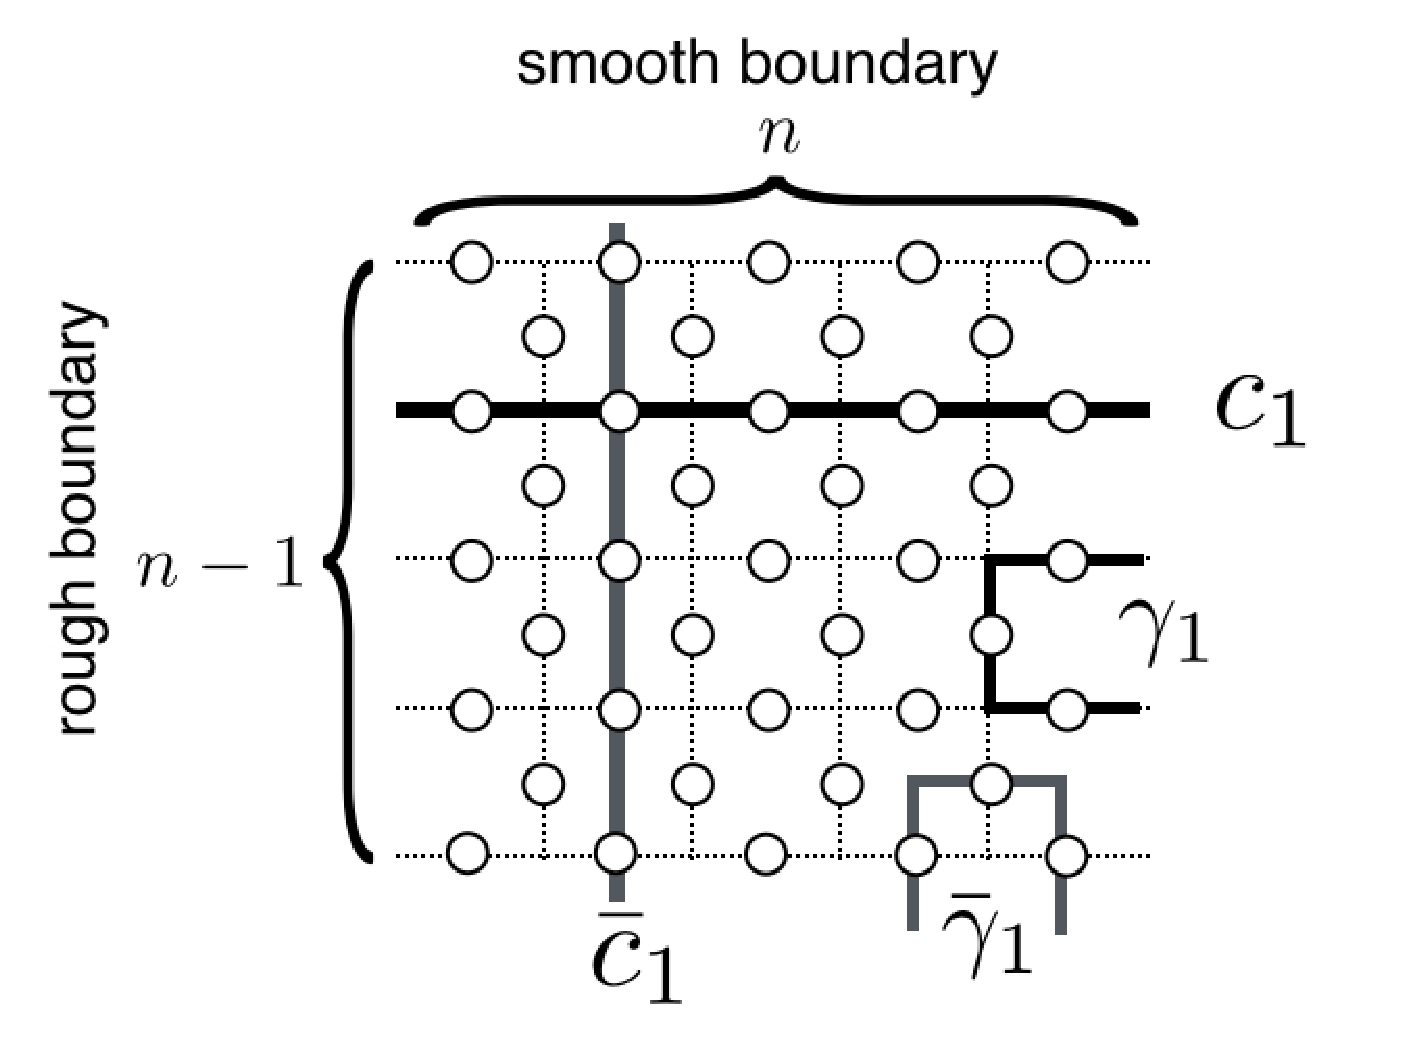
\includegraphics[width=90mm]{fig58.eps}
%
% If not, use
%\picplace{5cm}{2cm} % Give the correct figure height and width in cm
%
\caption{A planar surface code. 
Top and bottom are smooth boundaries consisting of three-qubit star operators. 
Left and right are rough boundaries consisting of three-qubit plaquette operators. 
At the boundary, we can define sets of 1-chains $\Gamma _1 = \{ \gamma _1 \} \in C_1$ and $\bar \Gamma _1 = \{ \bar \gamma _1 \} \in \bar C_1$ for the primal and dual lattices, respectively, by which the relative homology is defined.}
\label{fig58}       % Give a unique label
\end{figure}
%%%%%%%%%%%%%%%%%%%%%%%%%%%
%%%%%%%%%%%%%%%%%%%%%%%%%%%
The periodic boundary condition might be hard to implement in experiments.
We can also define a surface code on a planar $n\times (n-1)$ square lattice with an appropriate boundary condition as shown in Fig.~\ref{fig58}.
The top and bottom boundaries consist of three-qubit star operators, which we call smooth boundaries, because they are complete plaquette operators.
On the other hand, the left and right boundaries consist of three-qubit plaquette operators, which we call rough boundaries.
The $X$ operators on a dual 1-chain can terminate at the smooth boundary, while the $Z$ operators on a 1-chain can terminate at the rough boundary.
Thus, we should use a relative homology to define logical operators, where two chains $c_i$ and $c'_i$ are said to be (relative) homologically equivalent iff 
$c'_i = c_i + \partial c_{i+1} + \gamma_i$ with $\gamma _i \in \Gamma _i \subset C_i$.
In this case, $\Gamma _1$ is chosen, specifically, to be the vector space
spanned by the set of 1-chains each of which consists of three edges corresponding to the three-qubit plaquette operator at the top and bottom smooth boundaries.
Similarly, we also define $\bar \Gamma _1$ at the left and right rough boundaries of the dual lattice.
Because $Z(\gamma _1)$ and $X(\bar \gamma _1)$ are both stabilizer operators, if the shapes of two logical operators are homologically equivalent, their actions on the code state are the same.
The number of edges, faces, and vertices are now $|E|=2n^2 -2n +1$, $|V|=n^2-n$, and $|F|=n^2-n$.
Thus, the stabilizer subspace is a 2D subspace.
We can define the logical operators $L_Z=Z(c_1)$ and $L_X=X(\bar c_1)$ using horizontal and vertical 1-chains $c_1$ and $\bar c_1$, as shown in Fig.~\ref{fig58}.

\begin{figure}[t]
\centering
%\sidecaption
% Use the relevant command for your figure-insertion program
% to insert the figure file.
% For example, with the option graphics use
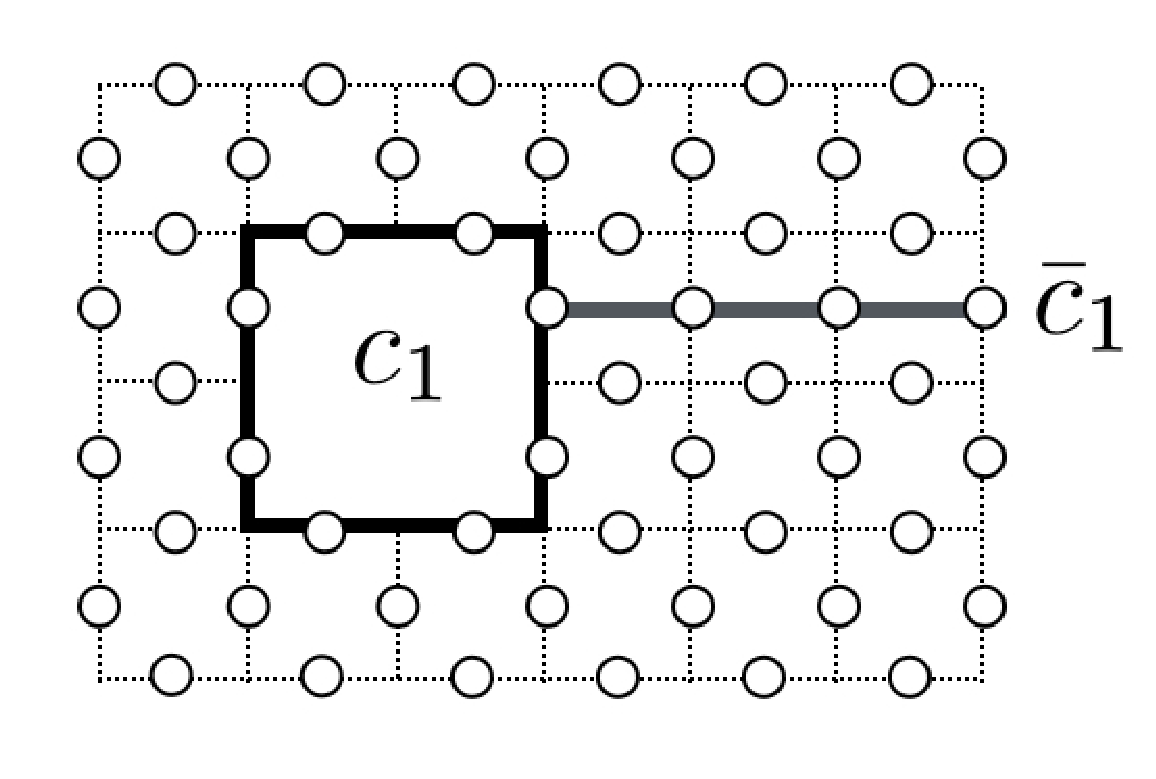
\includegraphics[width=90mm]{fig59.eps}
%
% If not, use
%\picplace{5cm}{2cm} % Give the correct figure height and width in cm
%
\caption{A planar surface code with a defect. 
The stabilizer generators are not defined  inside a defect, which provides a nontrivial cycle wrapping around it.}
\label{fig59}       % Give a unique label
\end{figure}
%%%%%%%%%%%%%%%%%%%%%%%%%%%
%%%%%%%%%%%%%%%%%%%%%%%%%%%
If one chooses all boundaries smooth, the stabilizer state is uniquely defined, and hence there is no logical degree of freedom.
By punching a hole, we can introduce a defect on the surface, whereby we can define a nontrivial cycle for a logical $Z$ operator, as shown in Fig.~\ref{fig59}.
The logical $X$ operator can be chosen as a dual 1-chain that connects the defect and the smooth boundary, as shown in Fig.~\ref{fig59}.
As mentioned previously, the properties of the logical operators are the same if the corresponding 1-chains are homologically equivalent.


\section{Topological quantum error correction}
\label{Sec:TQEC}
\begin{figure}[t]
\centering
%\sidecaption
% Use the relevant command for your figure-insertion program
% to insert the figure file.
% For example, with the option graphics use
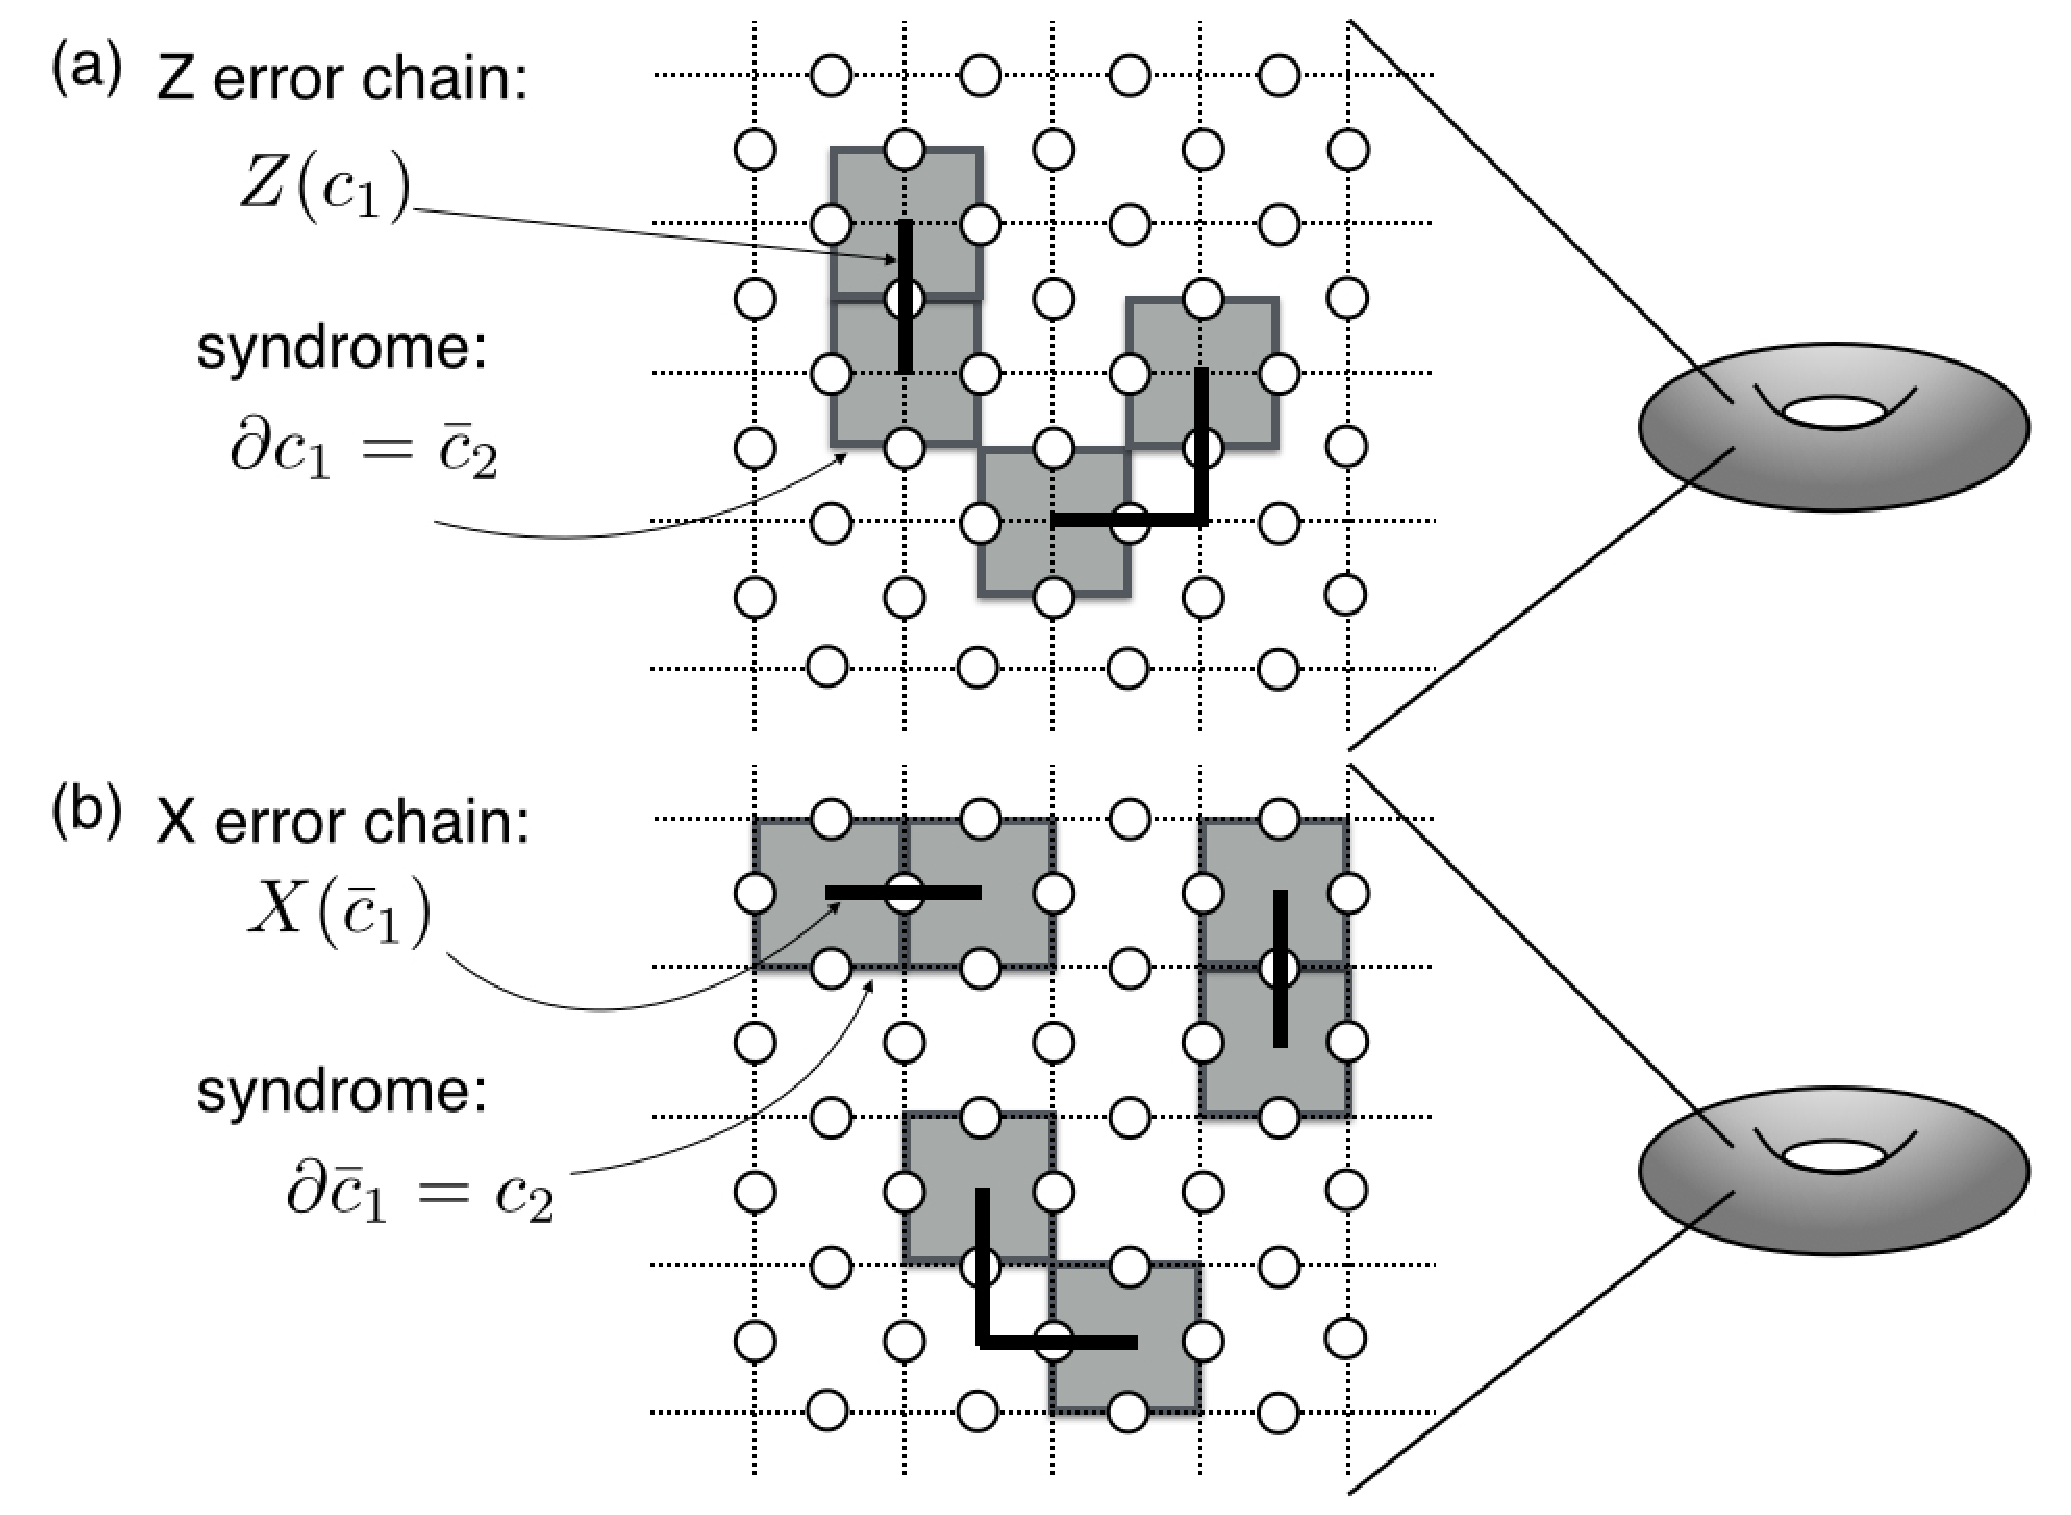
\includegraphics[width=110mm]{fig57.eps}
%
% If not, use
%\picplace{5cm}{2cm} % Give the correct figure height and width in cm
%
\caption{(a) A $Z$ error chain $Z(c_1)$ is detected at the boundary $\partial c_1$.
The eigenvalue of the stabilizer generator $B_k$ on the face $\bar f_k \in \bar c_2 =\partial c_1$ becomes -1. 
(b)  An $X$ error chain $X(\bar c_1)$ is detected at the boundary $\partial \bar c_1$.
The eigenvalue of the stabilizer generator $A_m$ on the face $f_m \in  c_2 =\partial \bar c_1$ becomes -1. }
\label{fig57}       % Give a unique label
\end{figure}
%%%%%%%%%%%%%%%%%%%%%%%%%%%
%%%%%%%%%%%%%%%%%%%%%%%%%%%
Let us return to the surface code on the torus to explain how errors are corrected.
There are $2^{2n^2-2}$ orthogonal subspaces, the so-called syndrome subspaces, each of which is an eigenspace of the stabilizer generators and has the same structure as the code space.
These orthogonal subspaces are utilized to identify the location of errors and to infer a recovery operation.
Suppose the $X$ and $Z$ errors $X(\bar c_1^{e})$ and $Z(c_1^{e})$, defined by error 1-chains $\bar c_1^{e}$ and $c_1^{e}$, respectively, occur on the surface code, as shown in Fig.~\ref{fig57}.
The code state is now mapped into one of the orthogonal subspaces.
From Eq.\ (\ref{eq:comm_rep}), $X(\bar c_1^{e})$ and $Z(c_1^{e})$ anticommute with $A_m$ and $B_k$ on the face $f_m \in \partial \bar c_1^e$ and vertex $v_k \in \partial c_1^e$.
Thus, the orthogonal subspace is specified by error syndromes 
\begin{eqnarray}
\partial \bar c_1^{e} \equiv c_2^{s}, \;\;\; \partial c_1^{e} \equiv c_0^{s}.
\end{eqnarray}
More precisely, the eigenvalues with respect to the stabilizer generators $A_m$ and $B_k$ are given by $(-1)^{z^s_m}$ and $(-1)^{z^s_k}$, where $c_2^{s}=\sum _m {z^s_m} f_m$ and $c_0^{s}=\sum _k z_k^s v_k$ (see Fig.~\ref{fig57}), respectively.
Error correction is the task of finding recovery 1-chains $\bar c_1^r$ and $c_1^{r}$ such that $\partial (\bar c_1^e + \bar c_1^r)=0$ and $\partial (c_1^e +  c_1^r)=0$,
meaning that the state is returned into the code space by applying $X(\bar c_1^r)$ and $Z(c_1^r)$, respectively.
Below we will, for simplicity, explain only how to correct the $Z$ errors, but the extension to the $X$ errors is straightforward.


Suppose each $Z$ error occurs with an independent and identical probability $p$.
Conditioned on the error syndrome $c_0^s=\partial c_1^e$, the posterior probability of an error $Z(c_1)$ occurring with $c_1= \sum _l z_l e_l$ is written as
\begin{eqnarray}
P( c_1 | c_0^{s}) &=&\mathcal{N} \prod _{l }  \left( \frac{p}{1-p} \right) ^{z_l} \big |  _{ \partial c_1 =c_0^s }
\label{eq:posterior}
\end{eqnarray}
where $\mathcal{N}$ is a normalization factor.
One way to find a recovery chain is by maximizing the posterior probability 
\begin{eqnarray}
c_1^r \equiv {\rm arg} \max _{c_1} P( c_1 | c_0^{s}) ={\rm arg} \min_{c_1} \left( \sum _{l} z_l \right) |_{\partial c_1 = c_0^s},
\end{eqnarray}
where $c_1=\sum _l z_l e_l$.
As seen in the l.h.s., this corresponds to minimizing the number of errors $\sum _{l}z^r_l$ such that $ \partial c_1^r = c_0^s$.
Hence, this is called minimum distance decoding.
If $c_1^r +c_1^e$ is a trivial cycle, the error correction succeeds, because the net action $Z(c_1^r +c_1^e)$ after the recovery operation is identity on the code state as shown in Fig~\ref{fig60}.
If $c_1^r +c_1^e$ is a nontrivial cycle, the recovery operation results in the logical operation $Z(c_1^r+c_1^e)\sim L_Z$, i.e., a logical error.
\begin{figure}[t]
\centering
%\sidecaption
% Use the relevant command for your figure-insertion program
% to insert the figure file.
% For example, with the option graphics use
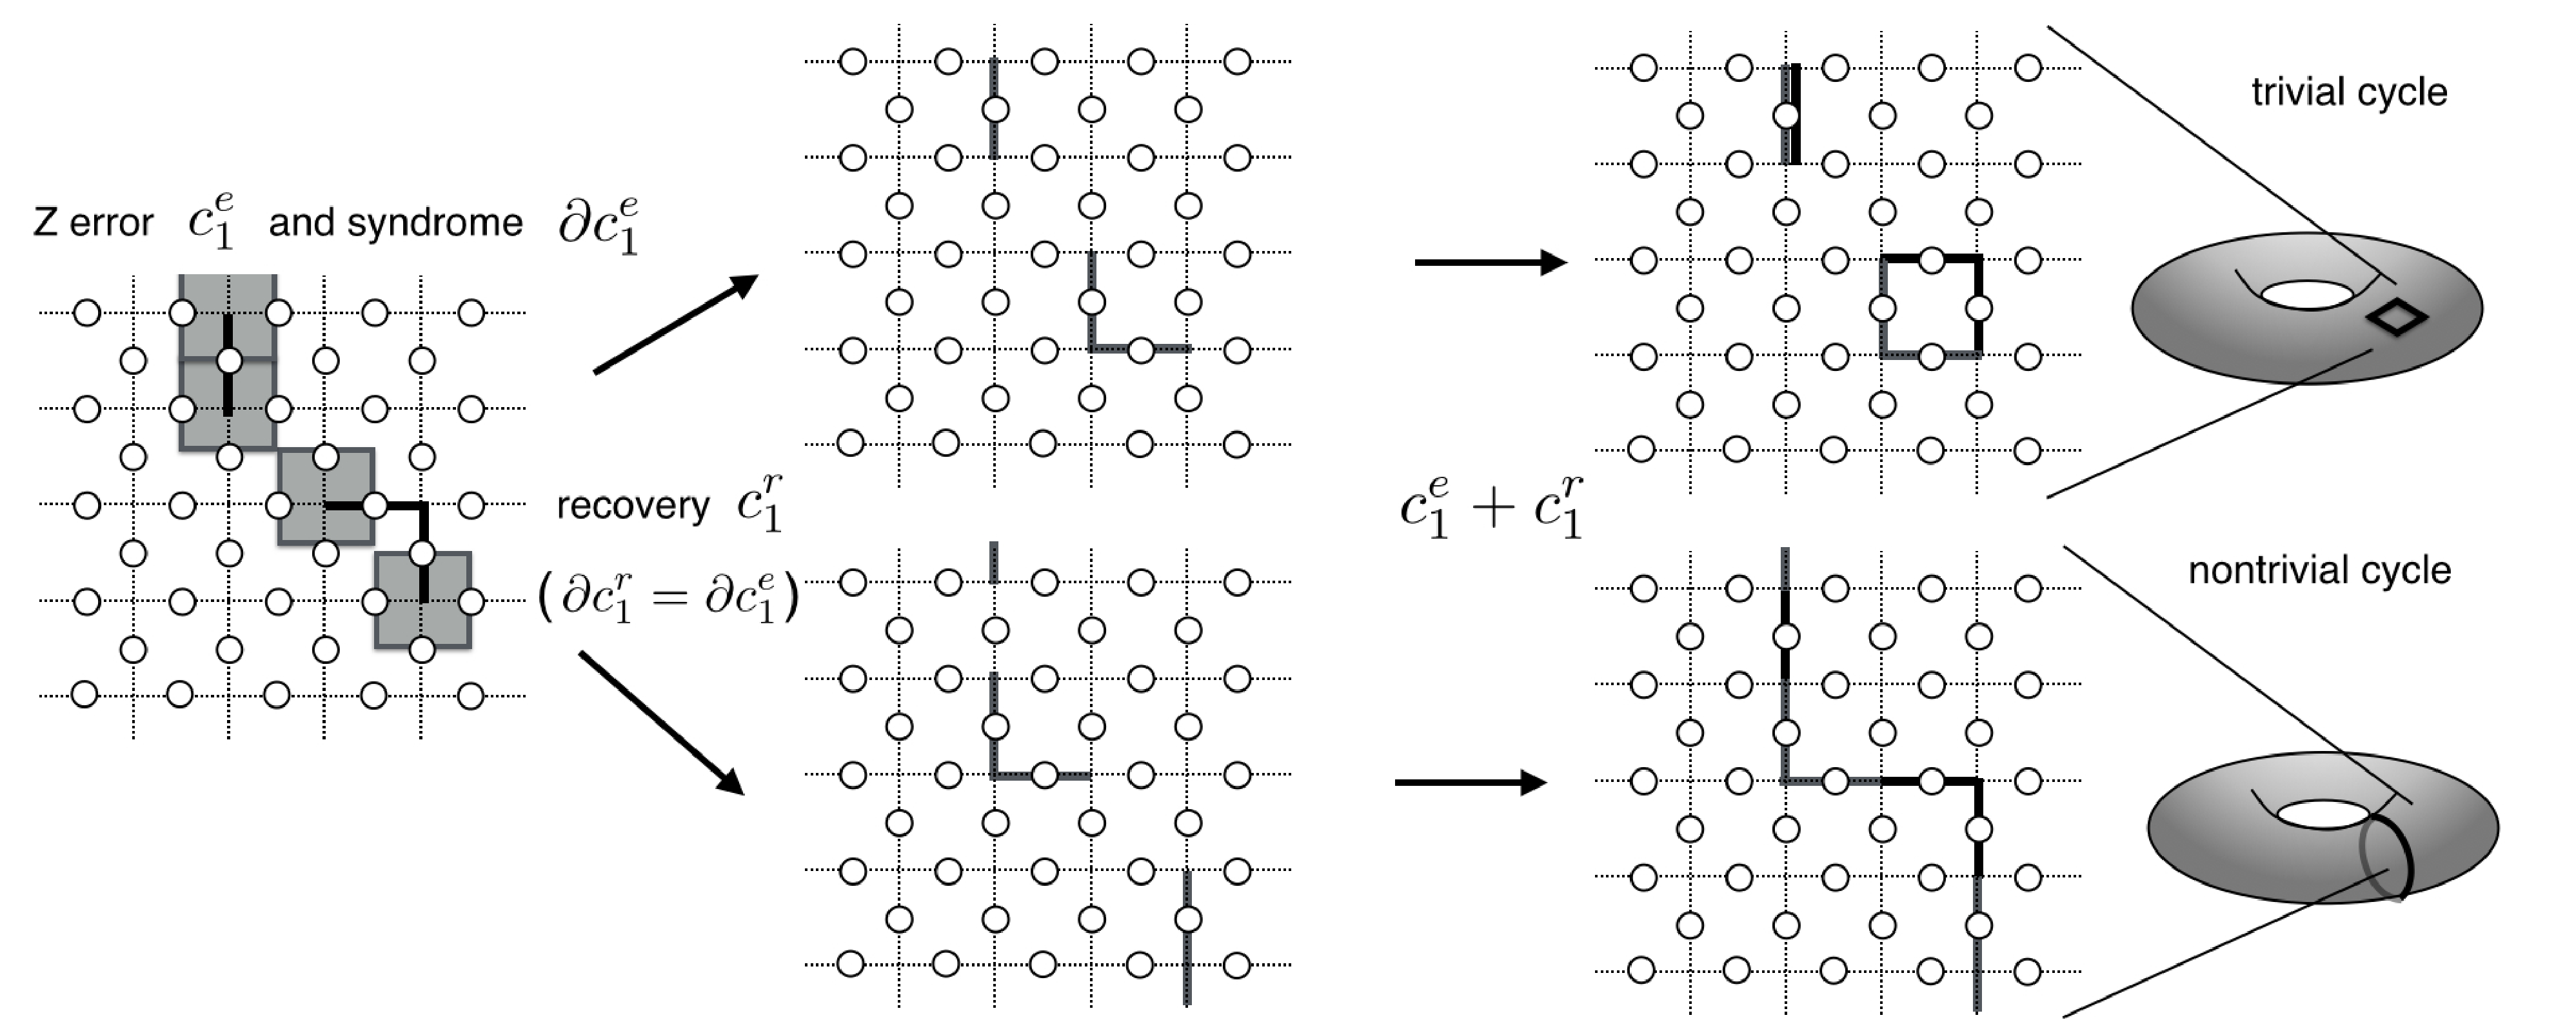
\includegraphics[width=150mm]{fig60.eps}
%
% If not, use
%\picplace{5cm}{2cm} % Give the correct figure height and width in cm
%
\caption{ From left to right, error chain $Z(c_1^e)$, recovery chain $Z(c_1^r)$ with $c_1^r=c_0^s$, and net actions $Z(c_1^r + c_1^e)$.
If $c_1^r + c_1^e$ is a trivial cycle (top), error correction succeeds. 
If $c_1^r + c_1^e$ is a non-trivial cycle (bottom), the error correction results in a logical error. }
\label{fig60}       % Give a unique label
\end{figure}

Minimum distance decoding is hard in general, because it can be mapped into an integer programing problem, which is NP-hard~\cite{DecodingNP,DecodingNP2,DecodingSharpP}. 
However, in the present case, there is a nice geometrical property that makes the decoding problem feasible.
The condition $ \partial c_1 = c_0^s$ and $\min _{c_1}$ read 
that it is sufficient to find a 1-chain that connects pairs of two vertices in $c_0^s$ with a minimum Manhattan length.
There is a classical polynomial time algorithm to do such a task, the so-called minimum-weight perfect matching (MWPM)\index{minimum-weight perfect matching, MWPM} algorithm of Edmonds~\cite{Edmonds,Barahona,Cook99}.
The algorithm scales like $O(n^6)$, with $n$ being the linear length of the lattice and with the fixed error probability $p$.
Typical examples of the error chain $c^e_1$ and the error plus recovery chain $c^e_1+e^r_1$ are shown in Fig.~\ref{fig66} for each $p=0.05$ (b), $p=0.10$ (c), and $p=0.15$ (d).
\begin{figure}[t]
\centering
%\sidecaption
% Use the relevant command for your figure-insertion program
% to insert the figure file.
% For example, with the option graphics use
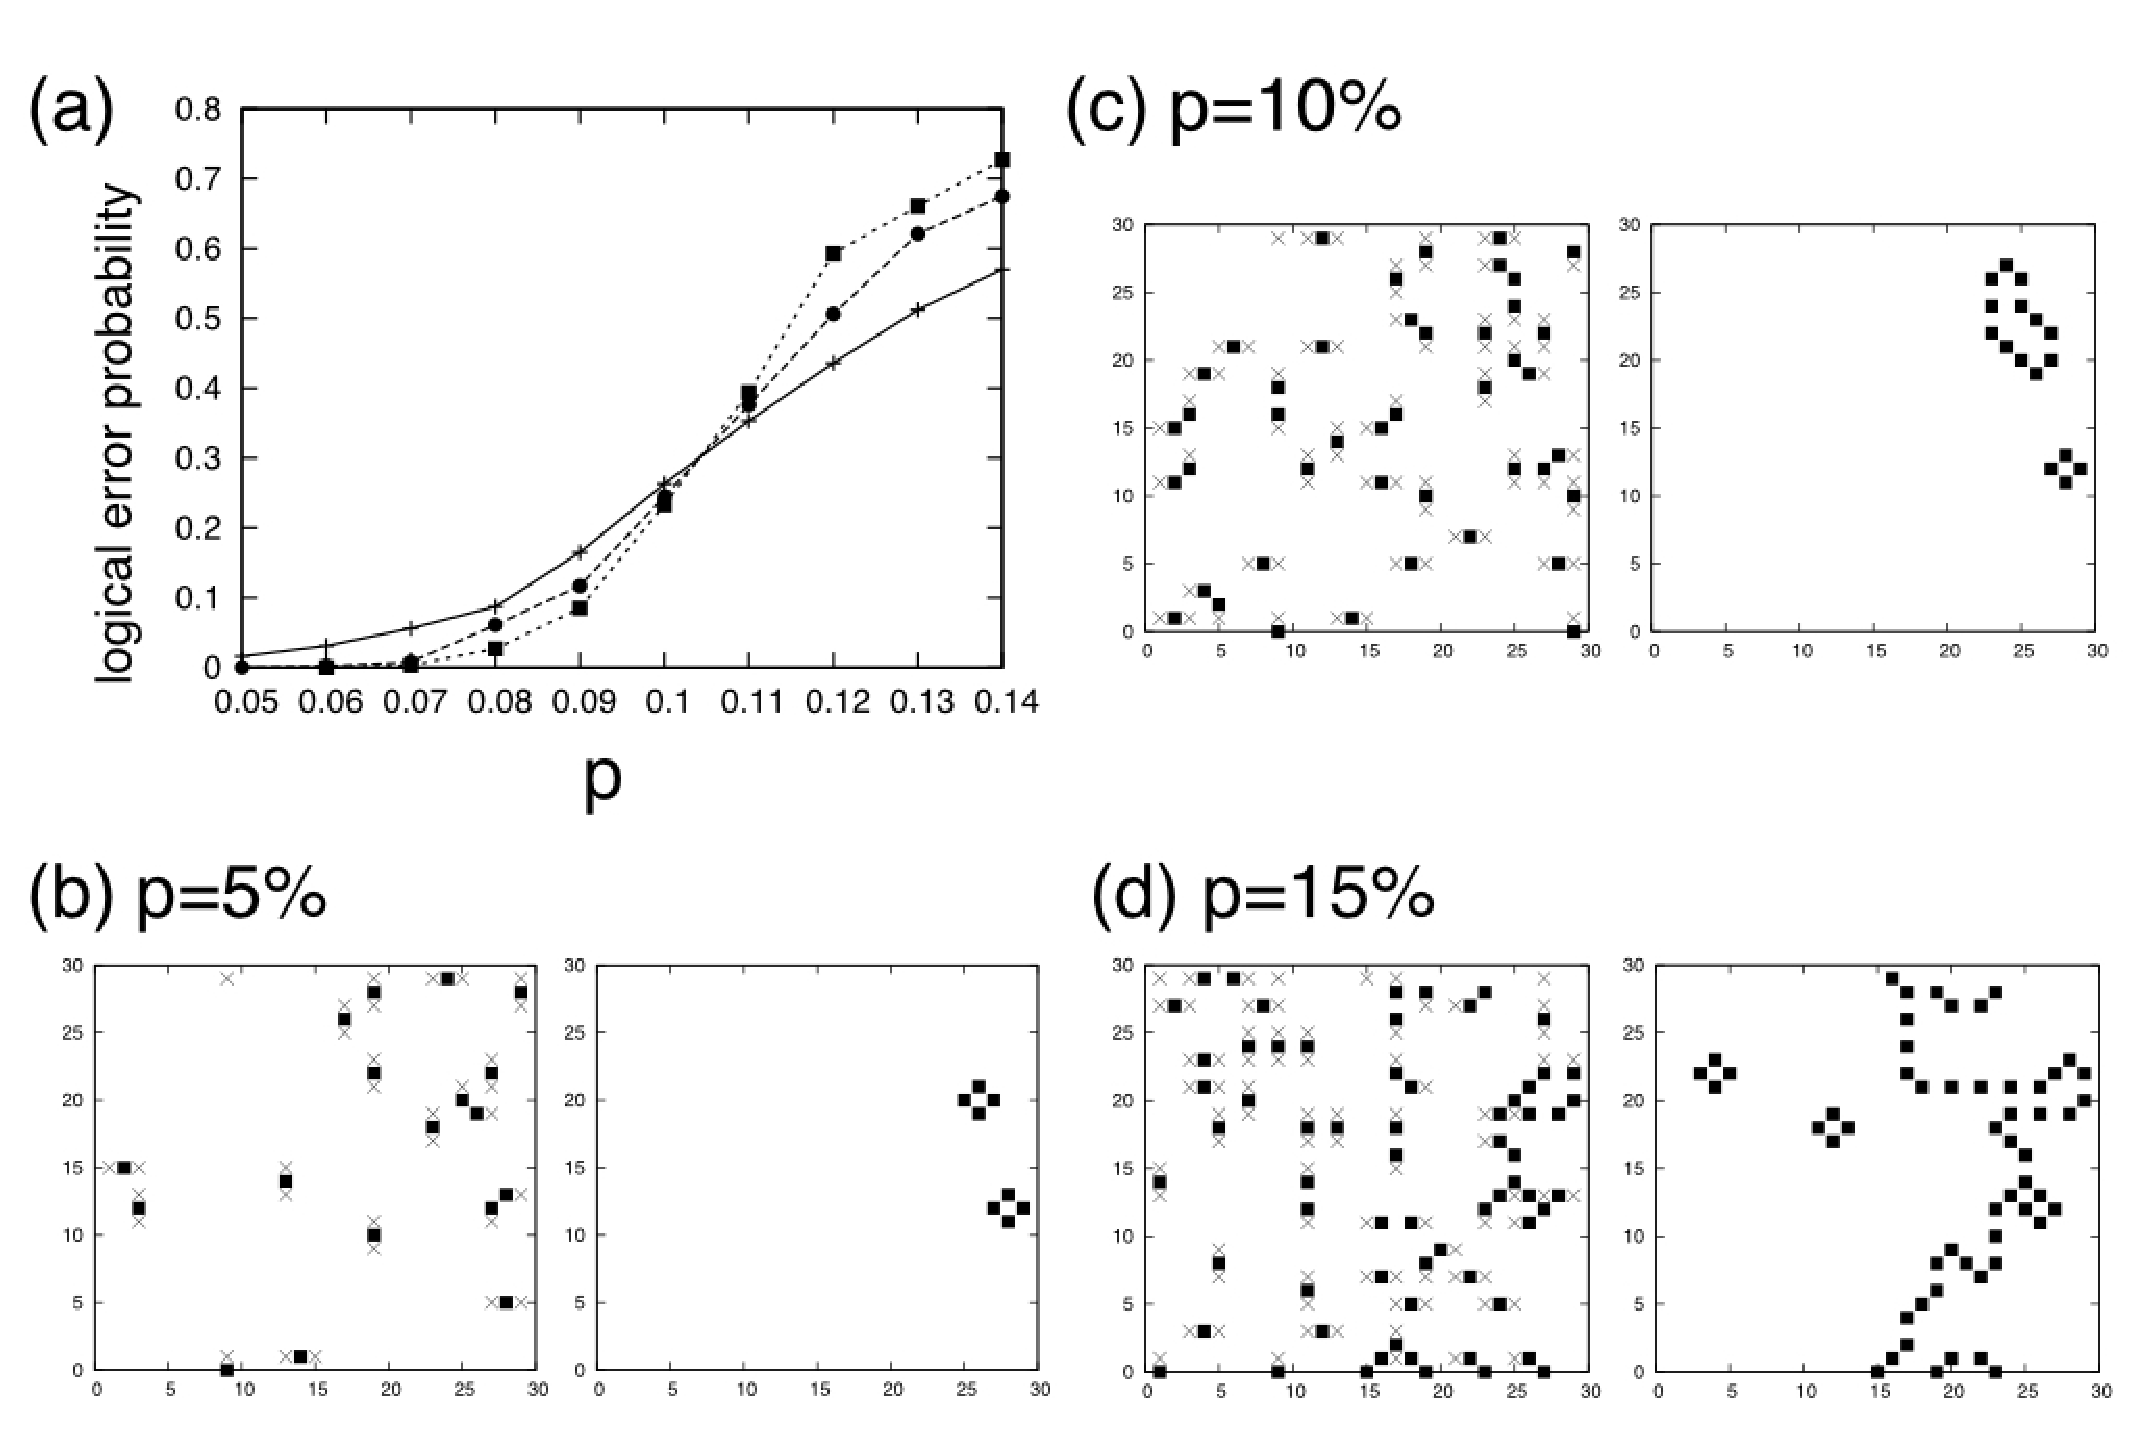
\includegraphics[width=130mm]{fig66.eps}
%
% If not, use
%\picplace{5cm}{2cm} % Give the correct figure height and width in cm
%
\caption{(a) The logical error probability is plotted as a function of the physical error probability $p$. 
Error chains $c_1^e$ and error plus recovery chains $c_1^e+c_1^r$ for $p=0.05$ (b), $p=0.10$ (c), and $p=0.15$ (d).}
\label{fig66}       % Give a unique label
\end{figure}
Here, we employ an implementation of MWPM, blossom V~\cite{Kolmogorov}.
The higher the physical error probability is, the longer the error plus recovery chain becomes.
For a high physical error probability $p=0.15$, the error plus recovery chain becomes a large cycle, and unfortunately results in a logical error. 
Such a logical error probability is plotted as a function of the physical error probability $p$ in Fig.~\ref{fig66} (a) for each $n=10$ (solid line), $n=20$ (dashed line), and $n=30$ (dotted line).
If the error probability is sufficiently smaller than a threshold value, the logical error probability decreases for increasing $n$.
The threshold value for decoding by the MWPM algorithm has been estimated to be 10.3\% (MWPM)~\cite{Dennis,Wang}.

The minimum distance decoding with MWPM is not optimal for our purpose, i.e., making the logical error probability as small as possible.
An error correction with another recovery chain $c_1^{r'}$, for which $c^e_1+c^{r'}_1$ belongs to the same homology class as $c^e_1+c^r_1$, provides exactly the same result.
We may use such a recovery chain $c_1^{r'}$ to correct the error.
Thus, we should maximize, not each posterior probability $p(c_1^{r}|c_0^s)$, but a summation of it over the same homology class.
This problem originated from the degeneracy of the surface code, where each syndrome is assigned not uniquely, but for many error instances.
A prototypical example of an error syndrome,
for which we should consider not olny the weight of errors,
but also combinatorics (an entropic effect) of the error configurations,
is shown in Fig.~\ref{fig61}.
\begin{figure}[t]
\centering
%\sidecaption
% Use the relevant command for your figure-insertion program
% to insert the figure file.
% For example, with the option graphics use
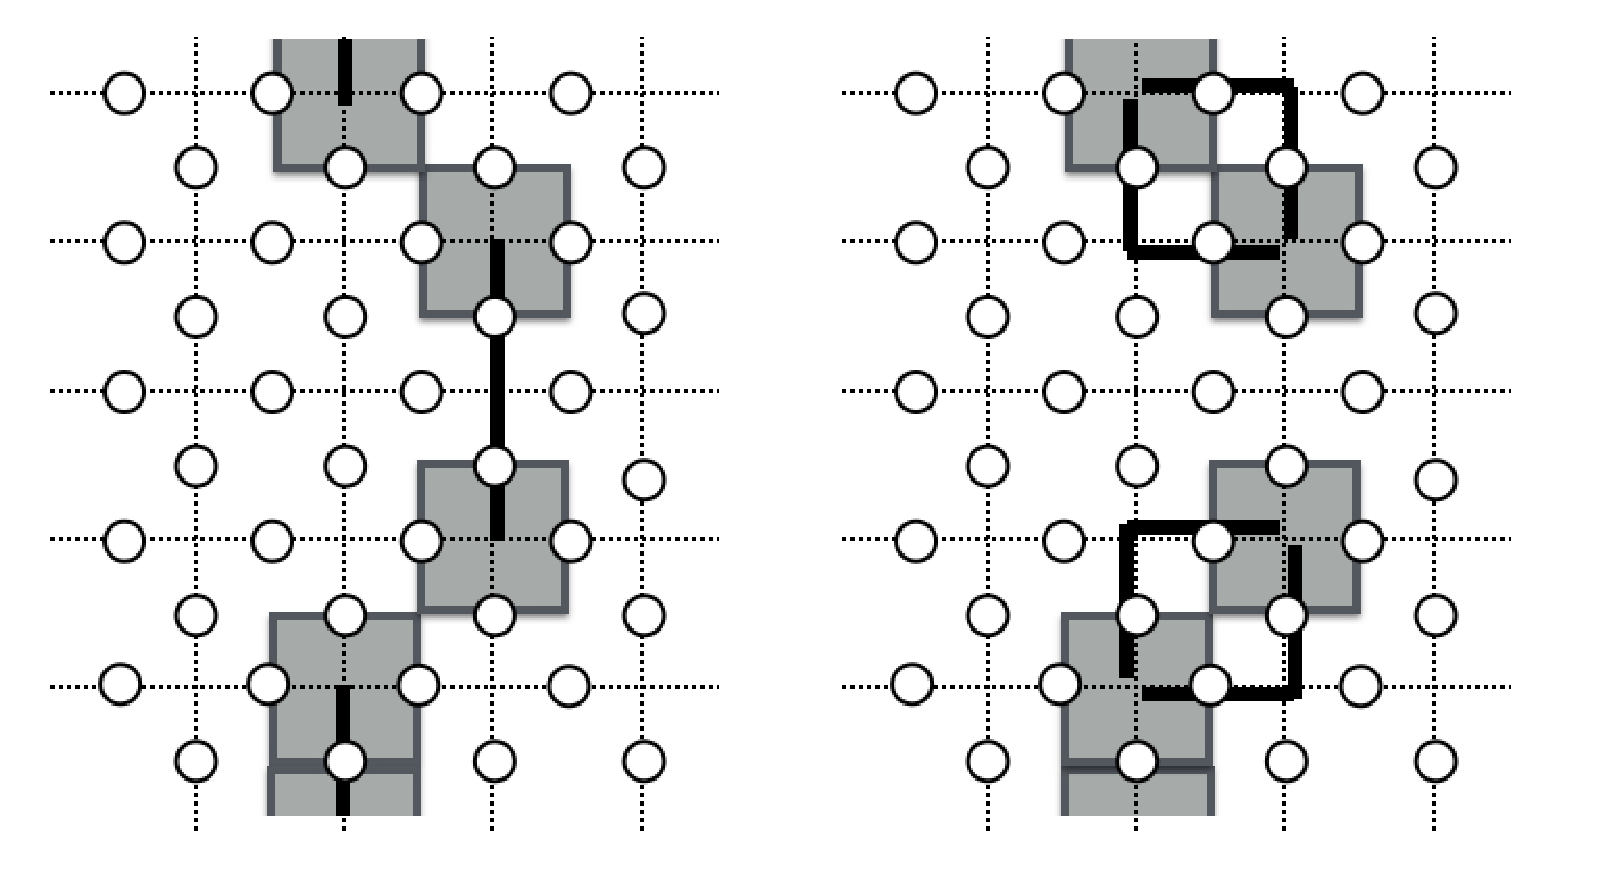
\includegraphics[width=100mm]{fig61.eps}
%
% If not, use
%\picplace{5cm}{2cm} % Give the correct figure height and width in cm
%
\caption{Suppose the top and bottom boundaries are connected by a periodic boundary condition. 
The minimum-weight error is shown in the left panel. 
The error shown in the right panel is not minimum-weight but has a fourfold degeneracy. 
The recovery chain should be chosen by comparing the total error probabilities $p^3$ and $4 \times p^4$.   }
\label{fig61}       % Give a unique label
\end{figure}

Denoting the homology class by $h_i$, the posterior probability for a homology class $h_i$ is given by
\begin{eqnarray}
p_i =\sum _{c_1^{r'}| c_1^r+c_1^{r'}\in h_i} P( c_1^{r'} | c_0^{s}),
\label{eq:prob_homo}
\end{eqnarray}
where $c_1^{r}$ is a recovery chain satisfying $\partial c_1^r = c_0^s$ and chosen arbitrarily as a reference frame, and the summation is taken over all 1-chains $c_1^{r'}$ such that $c_1^r + c_1^{r'}$ belongs to the homology class $h_i$.

The posterior probability may be rephrased by using the stabilizer language as follows (see also Appendix~\ref{Ap:Decode}).
Let $\mathcal{G}$ and $\mathcal{L}$ be the stabilizer and logical operator groups, respectively.
For a given error syndrome $c_0^{s}$, we define the recovery operator $Z(c_1^{r})$ a priori, such that the erroneous state is returned into the code space. 
We can decompose an arbitrary error operator $Z(c_1^e)$, providing the syndrome $c_0^{s}$, into 
\begin{eqnarray}
Z(c_1^e) = Z(c_1^{r}) G L_i,
\label{eq:decomposition}
\end{eqnarray}
where $G \in \mathcal{G}$ and $L_i \in \mathcal{L}$ are a stabilizer and logical operator, respectively.
The posterior probability of the logical operator $L_i$ is calculated by summing over all stabilizer operators $G \in \mathcal{G}$
\begin{eqnarray}
p_i = P (L_i| c_0^{s}) = \frac{1}{\mathcal{N}} \sum _{G \in \mathcal{G}} P[Z(c_1^{r}) G L_i ]. 
\end{eqnarray}
We choose the most likely homology class $h_i$ or, equivalently, the most likely logical operator $L_i$ that maximizes the probability $p_i =  P(L_i)$:
\begin{eqnarray}
L_{\bar i} \equiv {\rm arg}\max _{L_i}  P (L_i| c_0^{s}).
\end{eqnarray}
The error correction is completed by applying 
$L_{\bar i} Z(c^{r}_1)$, and the logical error probability 
is given by $1-p_{\bar i}$.

In the next section, we relate the posterior probability summed over the same homology class to a partition function of the random-bond Ising model.
The partition function of the Ising model on a planar graph with general coupling strengths (without magnetic fields) can be calculated in polynomial time using the Kasteleyn-Barahona algorithm with the Pfaffian method~\cite{Kasteleyn,Barahona,BravyiRaussendorf}.
Thus, the optimal decoding is also implemented by a polynomial time classical processing, though it takes more overhead than MWPM.
The threshold value for optimal decoding is also discussed in the next section.

Efficient decoding has been one of the most important issues for the realization of fault-tolerant quantum computing, because the coherence time of quantum information would be very short; a fast classical processing is essential.
Fowler {\it et al.} proposed an efficient decoding method based on MWPM~\cite{FowlerDecode}. 
Because a long error chain is exponentially suppressed, we can assign weights between each pairs of vertices having $-1$ eigenvalues according to their Manhattan length.
This allows us to reduce the number of edges from $O(n^4)$ to $O(n^2)$.
Moreover, the exponential suppression of longer error chains allows us to search the pairs within a local small region; matching a long-distance pair is exponentially rare.
Because the matching process employs almost exclusively local information, this algorithm can be parallelized to an O(1) average time per round. 

\begin{figure}[t]
\centering
%\sidecaption
% Use the relevant command for your figure-insertion program
% to insert the figure file.
% For example, with the option graphics use
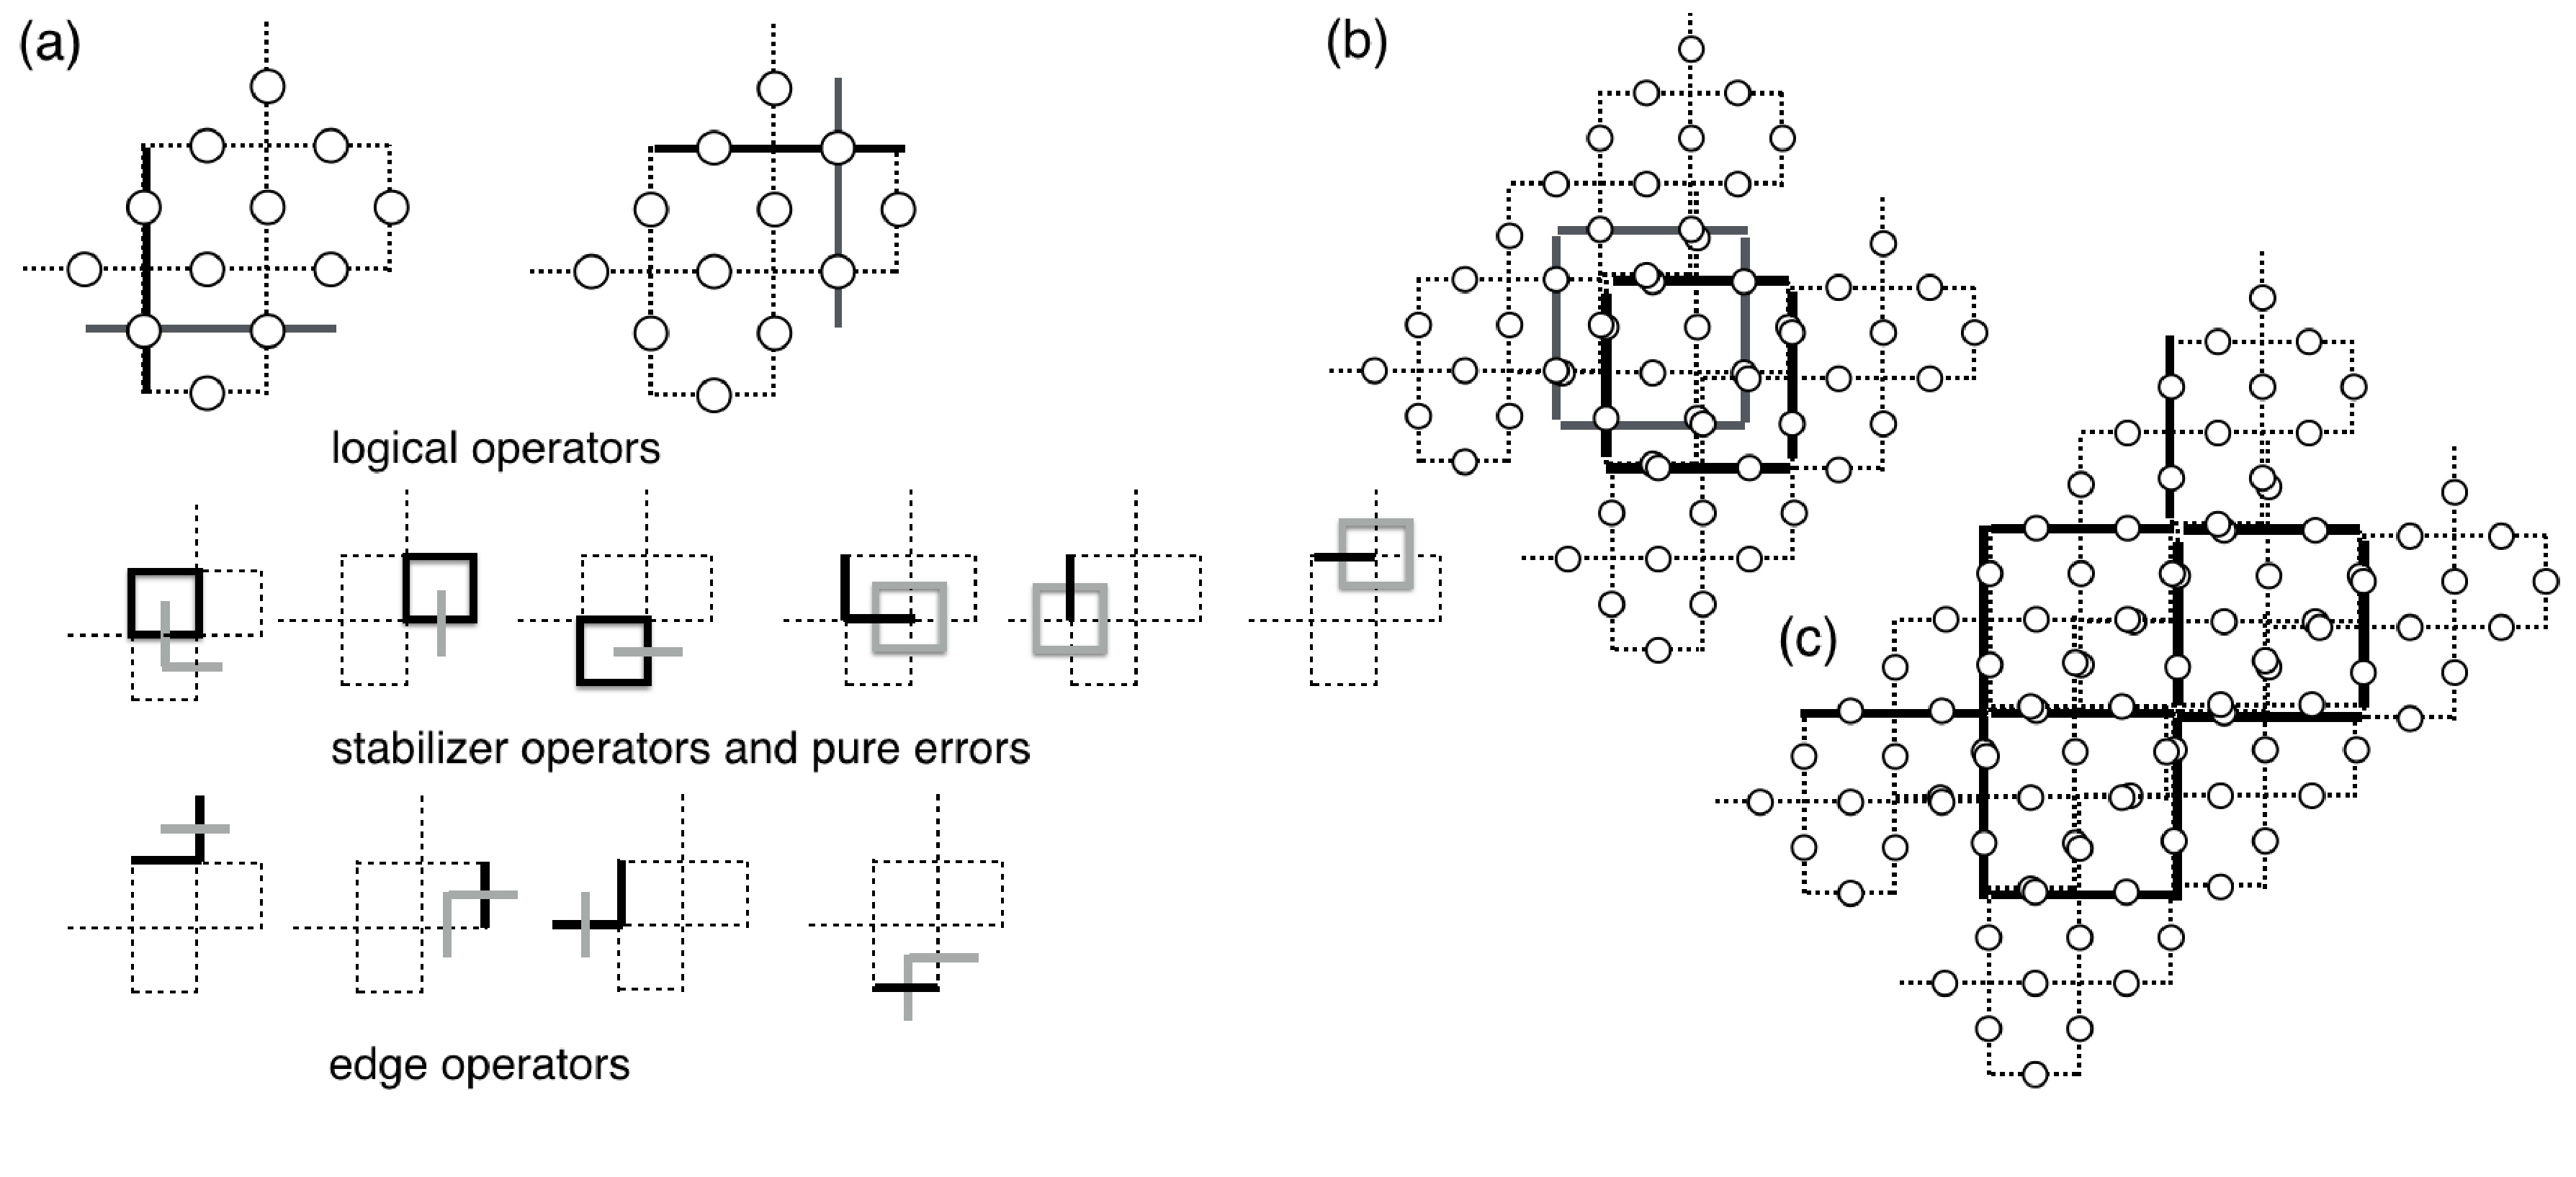
\includegraphics[width=150mm]{fig62.eps}
%
% If not, use
%\picplace{5cm}{2cm} % Give the correct figure height and width in cm
%
\caption{(a) A unit cell of the level-1 logical qubit. 
Two pairs of logical Pauli operators (top). 
The 6 stabilizer operators and the pure error operators,
each of which anticommutes with an stabilizer operator (middle).
The 4 pairs of edge operators.
These 12 pairs of mutually anti-commuting operators 
generate the Pauli group of the 12 qubits.
(b) Using the level-1 logical operators, the level-2 stabilizer generators are defined. 
(c) Using 12 level-1 logical qubits, a unit cell of the level-2 logical qubit is defined.}
\label{fig62}       % Give a unique label
\end{figure}
Another decoding method is using a renormalization technique~\cite{DuclosPoulin1,DuclosPoulin2}.
As explained in Appendix~\ref{Ap:Decode}, we can efficiently execute an optimal decoding on a concatenated quantum code by using a brief-propagation on a tree factor graph~\cite{Poulin06}.
Although the surface code itself does not have such a hierarchal structure, a renormalization technique is employed to introduce a hierarchal structure on the surface code~\cite{DuclosPoulin1,DuclosPoulin2}.

Using 12 qubits as a unit cell, we define a couple of level-1 logical qubits, as shown in Fig.~\ref{fig62} (a),
which include
2 pairs of logical operators $\mathcal{L}^{(1)}$, 
6 stabilizer generators $\mathcal{G}^{(1)}$. 
We define 6 pure error operators $\bar{\mathcal{G}}^{(1)}$
each of which anticommutes with a stabilizer generator
as shown in Fig.~\ref{fig62} (a) (middle).
Moreover, we define 4 pairs of anticommuting operators as shown in Fig.~\ref{fig62} (a) (bottom),
which we call edge operators $\mathcal{E}^{(1)}$, to generate the Pauli group of the 12 qubits.
Any Pauli operator $A$ on the unit cell
can be decomposed in terms of these operator,
\begin{eqnarray}
A = L^{(1)} G^{(1)} \bar G^{(1)} E^{(1)},
\end{eqnarray}
where $B^{(1)} \in \mathcal{B}^{(1)}$ for $B=L,G,\bar G, E$.
The pure error operator $\bar G^{(1)}$ is 
chosen uniquely according to the error syndrome $S^{(1)}$
to return the state into the code space.
(If a stabilizer generator $G_1$ has an eigenvalue $-1$,
then we employ $\bar G_1$, which anticommutes with $G_1$.)
From the error distribution $P(A)$, 
the posterior probability of the level-1 logical operator
is calculated by taking a marginal over $\mathcal{G}^{(1)}$ and $\mathcal{E}^{(1)}$,
\begin{eqnarray}
P(L^{(1)} | S^{(1)})=\sum _{G^{(1)} \in \mathcal{G}^{(1)}, E^{(1)} \in \mathcal{E}^{(1)}} P(A=L^{(1)} G^{(1)} \bar G^{(1)} E^{(1)}|S^{(1)}), 
\end{eqnarray}
which are utilized to model the error distribution at the level 2.

Similarly, a level-$k$ unit cell is defined 
by using 8 level-$(k-1)$ unit cells and the 12 pairs of 
the level-$(k-1)$ logical operators on them.
Similarly to the level-1 case,
we define the level-$k$ logical, stabilizer, pure error, edge operators.
At the highest level $k=l$,
we obtain the logical operators of the surface code.
For example, the level-2 stabilizer generators are shown in Fig.~\ref{fig62} (b).
A unit cell of the level-2 logical qubit is shown in Fig.~\ref{fig62} (c).

The posterior probability of the level-$k$
logical operator $P(L^{(k)} | S^{(k)})$ is calculated
using the posterior probabilities at the level $(k-1)$
by assuming that they are independent for each level-$(k-1)$ unit cell.
Under this assumption,
we can calculate the posterior probability $P(L^{(l)}|S^{(l)})$
conditioned on all error syndrome $S^{(l)}$ 
by using the belief propagation~\cite{Poulin06,DuclosPoulin1,DuclosPoulin2} 
(see Appendix ~\ref{Ap:Decode} for 
decoding the concatenated codes by using the belief propagation).
Then the maximization procedure over all logical operators
provide us a most likely logical operator,
\begin{eqnarray}
L^*= {\rm arg}\max _{L^{(l)}} P(L^{(l)} | S^{(l)}).
\end{eqnarray}
The level-$(k-1)$ unit cells share physical qubits with each other, and hence the conditional logical error probability is not independent 
for level-$(k-1)$ unit cells. 
If we employ a message passing in order to reweigh
the level-$(k-1)$ logical error probability as the error model 
for the level-$k$ unit cell,
we can further improve the approximation of $P(L^{(l)} | S^{(l)})$.
If the decoding process is done in parallel, the belief propagation takes $O(\log_2 (n))$ time, similar to the case of the concatenated code as explained in Appendix~\ref{Ap:Decode}.
Because the posterior probability is approximated, the decoding based on the renormalization is not optimal, but results in a reasonable threshold value,
$\sim 9\%$ for the independent $X$ and $Z$ error
and $\sim 15.2\%$ for the depolarizing error
(against $10.3\%$ and $15.5\%$ obtained by MWPM, respectively)
~\cite{DuclosPoulin1,DuclosPoulin2}.
The renormalization decoder can also be applied for an arbitrary topological code~\cite{BombinTopoStab}.


\section{Error correction and spin glass model}
\label{Sec:TQECandSpinGlass}
The behavior of the logical error probability in Fig.~\ref{fig66} suggests the existence of a critical phenomenon behind the error correction problem.
Indeed, there is a beautiful correspondence between quantum error correction on the surface code and a spin glass model, the so-called random-bond Ising model (RBIM)\index{random-bond Ising model, RBIM}~\cite{Dennis}.
More precisely, the posterior probability Eq.\ (\ref{eq:prob_homo}) of the logical operator is mapped into a partition function of the RBIM as seen below.

To solve the condition $\partial c_1 = c_0^s $ in Eq.\ (\ref{eq:posterior}), we rewrite the recovery chain as $c_1 = c_1^{r_k}+c_1^{t}$, where $c_1^{t}\in {\rm Img}(\partial _2)$ is a trivial cycle.
$c_1^{r_k}$ is further decomposed into $c_1^{r_k} = c_1^e+ c_1^{(k)}$, where $c_1^e$ determines the actual location of errors, and $c_1^{(k)}$ is a (nontrivial) cycle belonging to the homology class $h_k$.
Note that this decomposition corresponds to Eq.\ (\ref{eq:decomposition}).
The posterior probability is rewritten as
\begin{eqnarray}
P( c_1  | c_0^{s}) &=&\mathcal{N} \prod _{l }  \left( \frac{p}{1-p} \right) ^{z_l^{t} \oplus z_l^{r_k}} \Bigl|_{c_1^{t} \in {\rm Img}(\partial _2)},
\end{eqnarray}
where $c_1^{\alpha}=z_l^{\alpha} e_l$, with $z_l^{\alpha} \in \{ 0,1\}$. 
In order to take the condition $c_1^{t} \in {\rm Img}(\partial _2)$
automatically, 
we introduce a gauge valuable $z_m^g \in \{ 0,1\}$ on each dual vertex $\bar v_m$
and a dual 0-chain $\bar c_0^{g} = \sum _m z_m^g \bar v^g_m$.
Any trivial cycle $c_1^{t}$ is replaced by the gauge valuables using the following relation
\begin{eqnarray}
z_l^t = \bigoplus _{\bar v_m \in \partial \bar e_l} z_m^g.
\end{eqnarray}
For example, if we choose $\bar c_0^{g} = \bar v_m$, we obtain $c_1^{t}= \partial f_m$.
(This corresponds to a multiplication of the face stabilizer generator defined on the face $f_m$.)
There is a one-to-one correspondence between a trivial cycle and a gauge dual 0-chain.
Using $c_0^g$ we can formally solve the condition 
$c_1^{t} \in {\rm Img}(\partial _2)$ in Eq.\ (\ref{eq:posterior}),
\begin{eqnarray}
P( c_1  | c_0^{s}) &=&\mathcal{N} \prod _{l }  \left( \frac{p}{1-p} \right) ^{ z_l^{r_k}\bigoplus _{\bar v_m \in\partial \bar e_l} z_m^g}.
\label{eq:gauge_trans}
\end{eqnarray}
The binary valuables $z_i\in \{ 0,1\}$ are transformed into spin variables $\sigma _i \in \{ +1,-1\}$ by $\sigma _i= (-1)^{z_i}$.
Moreover, we define a coupling constant $e^{-J} = \sqrt{p/(1-p)}$.
Then Eq.\ (\ref{eq:gauge_trans}) is rewritten as 
\begin{eqnarray}
P( c_1  | c_0^{s}) &=&\mathcal{N}' e ^{J \sum _l \sigma_l^{r_k}\sigma^g _{m(l)}\sigma^g _{m'(l)}},
\end{eqnarray}
where $\mathcal{N}'$ is a normalization factor and $m(l)$ and $m'(l)$ are end points of the edge $e_l$.
By changing the notation $l \rightarrow ij$ and $m(l), m'(l) \rightarrow i,j$, the posterior probability is reformulated as a Boltzmann factor of the $\pm J$ RBIM:
\begin{eqnarray}
P( c_1  | c_0^{s}) &=&\mathcal{N}' e ^{ \sum _{ij} J_{ij}^{(k)}\sigma^g _{i}\sigma^g _{j}},
\end{eqnarray}
where $J_{ij}^{(k)} = J\sigma _{ij}^{r_k}$.
On the edges where the errors are located, anti-ferromagnetic interactions are assigned.
The posterior probability of the logical operator Eq.\ (\ref{eq:prob_homo}) is calculated by taking summation over all gauge spin configurations (this corresponds to the summation over all stabilizer operators in Eq.\ (\ref{eq:prob_homo})):
\begin{eqnarray}
p_{k}&=& \sum _{c_1^{r'}| c_1^{r_k}+c_1^{r'} \in h_k} P( c_1^{r'}  | c_0^{s})
\\
&=& \sum _{c_1^{t} |  c_1^{t} \in {\rm Img}(\partial _2)} P( c_1^{r_k}+ c_1^{t}  | c_0^{s})
\\
&=&
\sum _{\{ \sigma _i^{g}\}} \mathcal{N}' e ^{ \sum _{ij} J_{ij}^{(k)}\sigma^g _{i}\sigma^g _{j}}.
\\
&=& \mathcal{N}' \mathcal{Z}(\{ J_{ij}^{(k)}\}),
\label{eq:logi_prob1}
\end{eqnarray}
where $\mathcal{Z}(\{ J_{ij}^{(k)}\})$ is the partition function of the $\pm J$ RBIM.

Let us consider the performance under this decoding by taking an average of the logarithm of $p_k$ over the error distribution, which corresponds to a sample average with respect to quenched randomness:
\begin{eqnarray}
\bar p^{\rm ln}_k \equiv [\ln (p_k)] &=& \sum _{c_1^{e}} P(c_1^{e}) p_k
\\
&=&
\sum _{\{ J_{ij}\}} P(\{ J_{ij}^{e} \}) \ln \mathcal{Z}(\{ J_{ij}^{(k)}\}) +\ln \mathcal{N}'
\\
&\equiv & -F_k + \ln \mathcal{N}', 
\label{eq:sample_ave}
\end{eqnarray}
where $[\cdot]$ indicates the sample average and $\bar p^{\rm ln}_k$ is the sample average of the logarithm of the logical error probability $p_k$.
The quenched randomness is determined by the error distribution
\begin{eqnarray}
P( J_{ij}^{e} ) =(1-p') \delta ( J_{ ij}^{e} -1 )+ p'\delta ( J_{ i  j}^{e} +1 ).
\end{eqnarray}
Note that $p$ is a parameter in the posterior probability and could be different from the actual error probability $p'$.
Of course, optimal decoding,
in the sense of Bayesian inference, is achieved by maximizing the posterior probability with a true error probability $p=p'$.
$F_0=-[\ln \mathcal{Z}(\{ J_{ij}^{(0)}\})]$ is the free-energy of the RBIM, while $F_k =-[\ln \mathcal{Z}(\{ J_{ij}^{(k)}\})]$ ($k=1,2,3$) is the free-energy with respect to the interactions $\{ J_{ij}^{(k)}\}$, where a domain wall of anti-ferromagnetic interactions corresponding to a cycle $c_1^{(k)}$ of a homology class $h_k$ is inserted.

\begin{figure}[t]
\centering
%\sidecaption
% Use the relevant command for your figure-insertion program
% to insert the figure file.
% For example, with the option graphics use
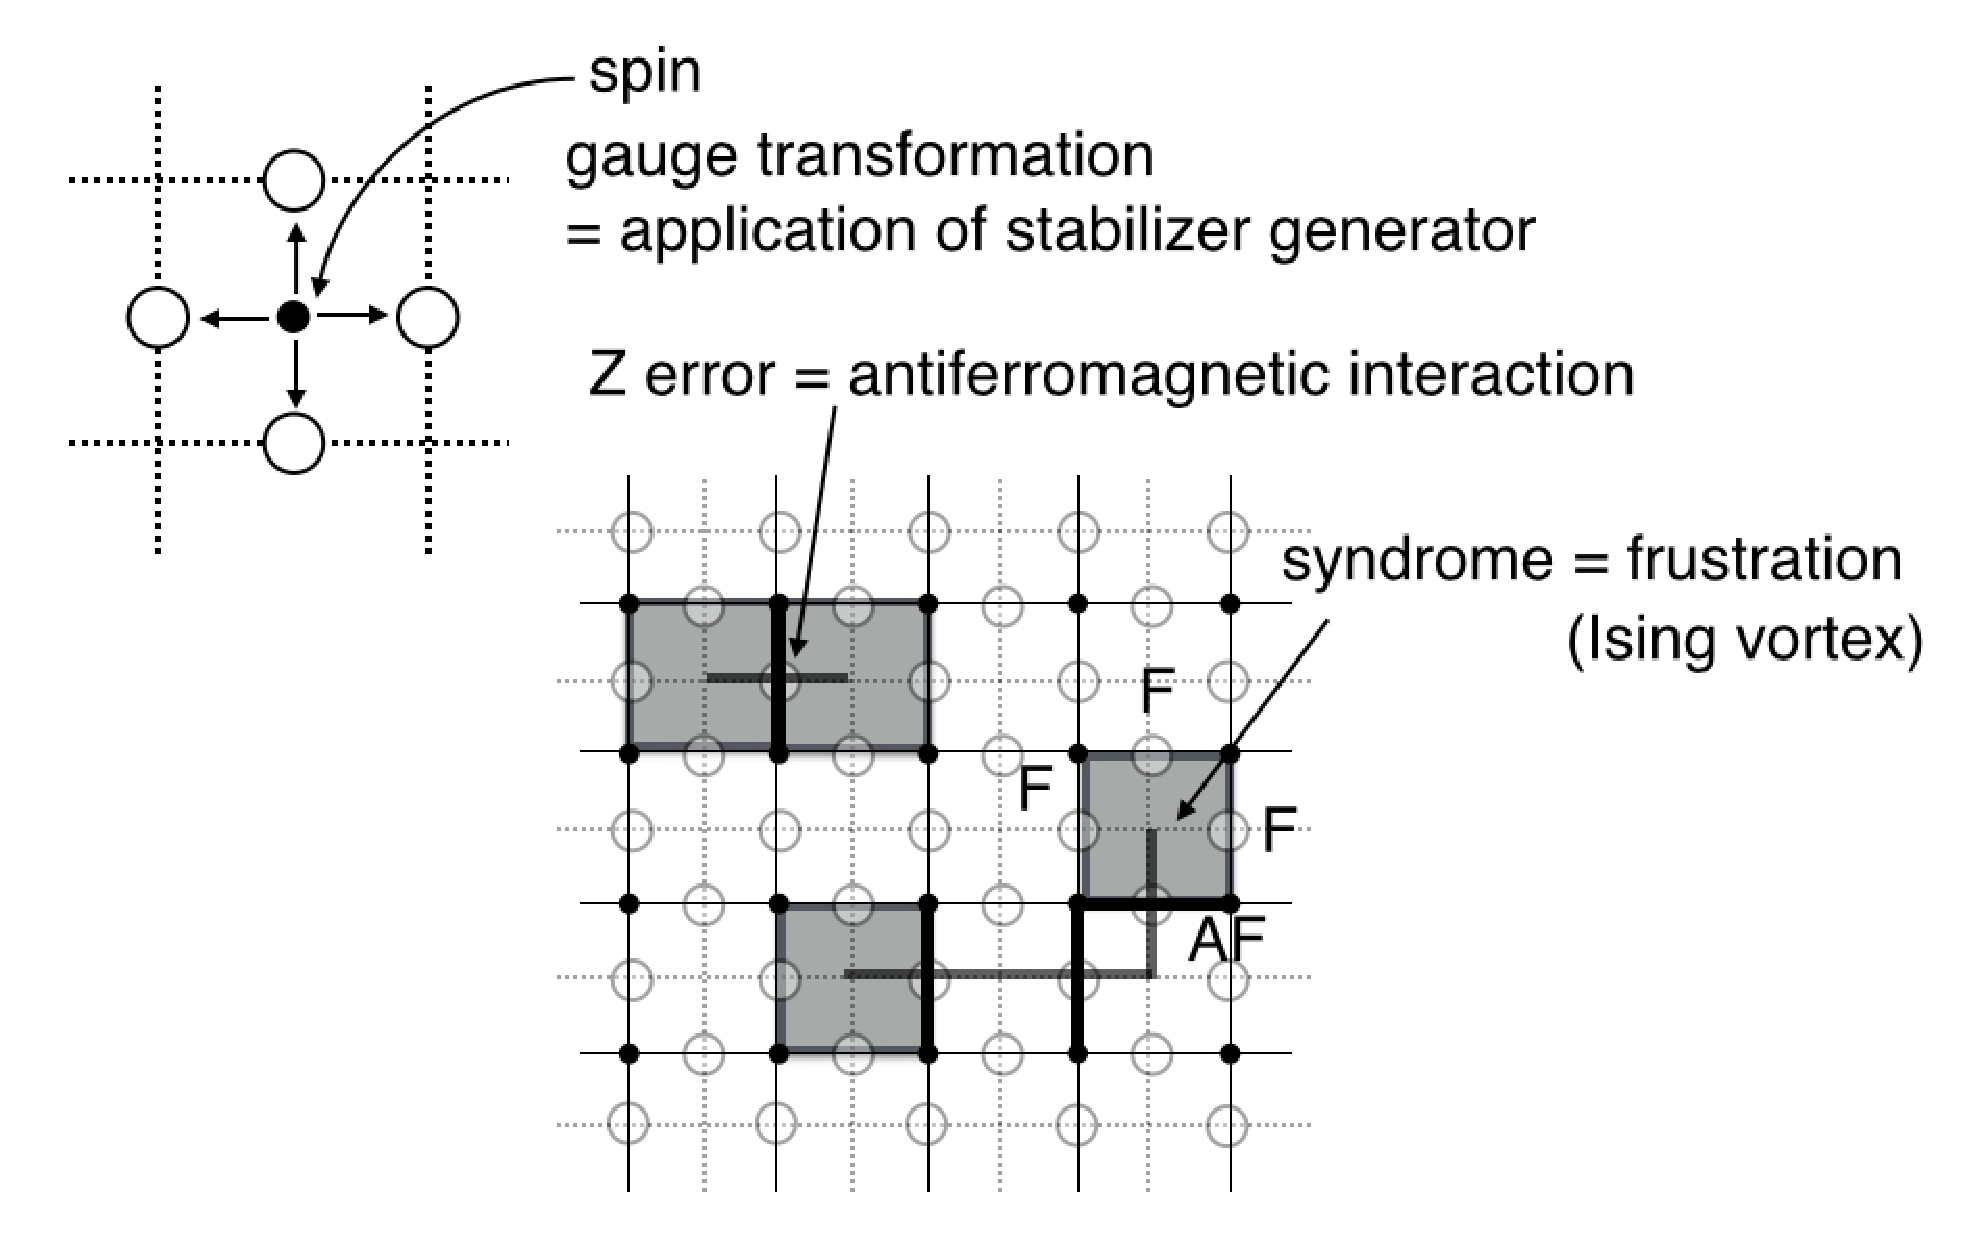
\includegraphics[width=130mm]{fig64.eps}
%
% If not, use
%\picplace{5cm}{2cm} % Give the correct figure height and width in cm
%
\caption{A gauge spin $\sigma ^g_f$ located at the face-center of a plaquette.
The distribution of anti-ferromagnetic interactions corresponds to the error chain $c_1^e$.
The error syndrome $c_0^s=\partial c_1^e$ corresponds to the distribution of frustrations. 
The ground state configuration is determined by a domain-wall consisting of excited domain-wall and anti-ferromagnetic bonds, both of which have frustrations at their end points.}
\label{fig64}       % Give a unique label
\end{figure}
From Eqs.\ (\ref{eq:logi_prob1}) and (\ref{eq:sample_ave}), the relation between quantum error correction and a spin glass model becomes apparent; the posterior probability of the logical operator is proportional to the partition function of RBIM, whose Hamiltonian is given by $H= - \sum _{ij} J_{ij}^{(k)} \sigma^g _i \sigma^g _j$.
The location of the $Z$ errors, represented by $J_{ij}^{(k)} = -1$, corresponds to the anti-ferromagnetic interaction due to disorder as shown in Fig.~\ref{fig64}
(see also Tab.~\ref{tab:ChainStabCode2}).
The error probability and the coupling strength (inverse temperature)
are related by $e^{-J} = \sqrt{p/(1-p)}$.
The error syndrome $c_0^s=\partial c_1^e$ corresponds to the distribution of frustrations of the Ising interactions and also the end points (Ising vortex) of the excited domain walls. 
\begin{figure}[t]
\centering
%\sidecaption
% Use the relevant command for your figure-insertion program
% to insert the figure file.
% For example, with the option graphics use
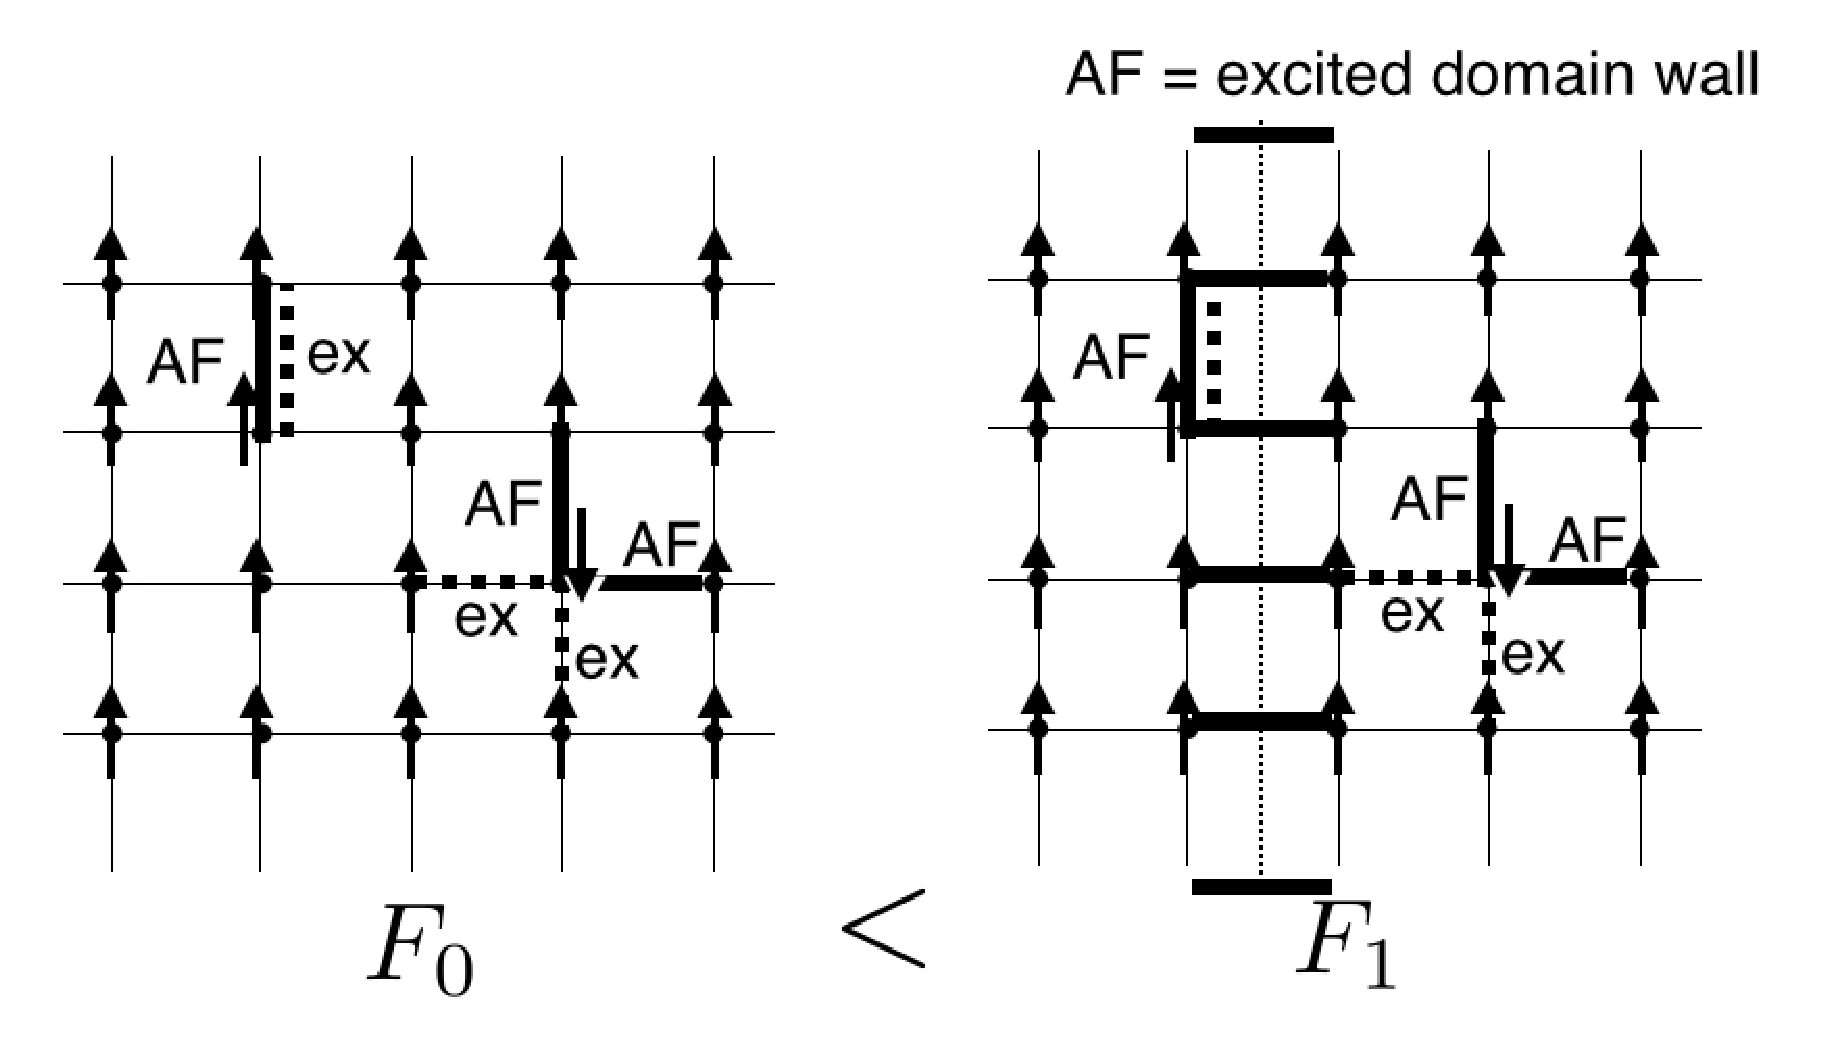
\includegraphics[width=120mm]{fig63.eps}
%
% If not, use
%\picplace{5cm}{2cm} % Give the correct figure height and width in cm
%
\caption{Examples of ground states in a ferromagnetic phase are shown for $\{ J_{ij}^{(k)}\}$ with $k=0,1$.
In the ferromagnetic case, the insertion of the anti-ferromagnetic bonds results in an excited domain-wall and hence increases the free energy (ground state energy at zero temperature).} 
\label{fig63}       % Give a unique label
\end{figure}
The probability of the homology class is expressed by the domain-wall free energy:
\begin{eqnarray} 
-(\bar p_k^{\ln} - \bar p_0^{\ln}) = {F_k-F_0}.
\label{eq:exponent}
\end{eqnarray}
If the physical error probability $p$ is smaller than the threshold value, $-\bar p _k^{\ln}$ ($k=1,2,3$) diverges in the large $n$ limit.
On the other hand, if $p$ is higher than the threshold value, $-\bar p _k^{\ln}$ ($k=0,1,2,3$) converges to $2\ln 2$ meaning the stored information becomes completely destroyed.
This non-analytical behavior also appeared in the r.h.s.\ of Eq.\ (\ref{eq:sample_ave}), i.e., the free-energy of RBIM.
Indeed, the difference between the free energies $\Delta =F_k - F_0$ is an order parameter, the so-called domain-wall free energy~\cite{Hukushima99}, for a ferromagnetic ordered phase.
The phase diagram of RBIM with respect to $J=(1/2)\ln [p/(1-p)] $) and $p'$ is shown in Fig.~\ref{fig65}.
\begin{figure}[t]
\centering
%\sidecaption
% Use the relevant command for your figure-insertion program
% to insert the figure file.
% For example, with the option graphics use
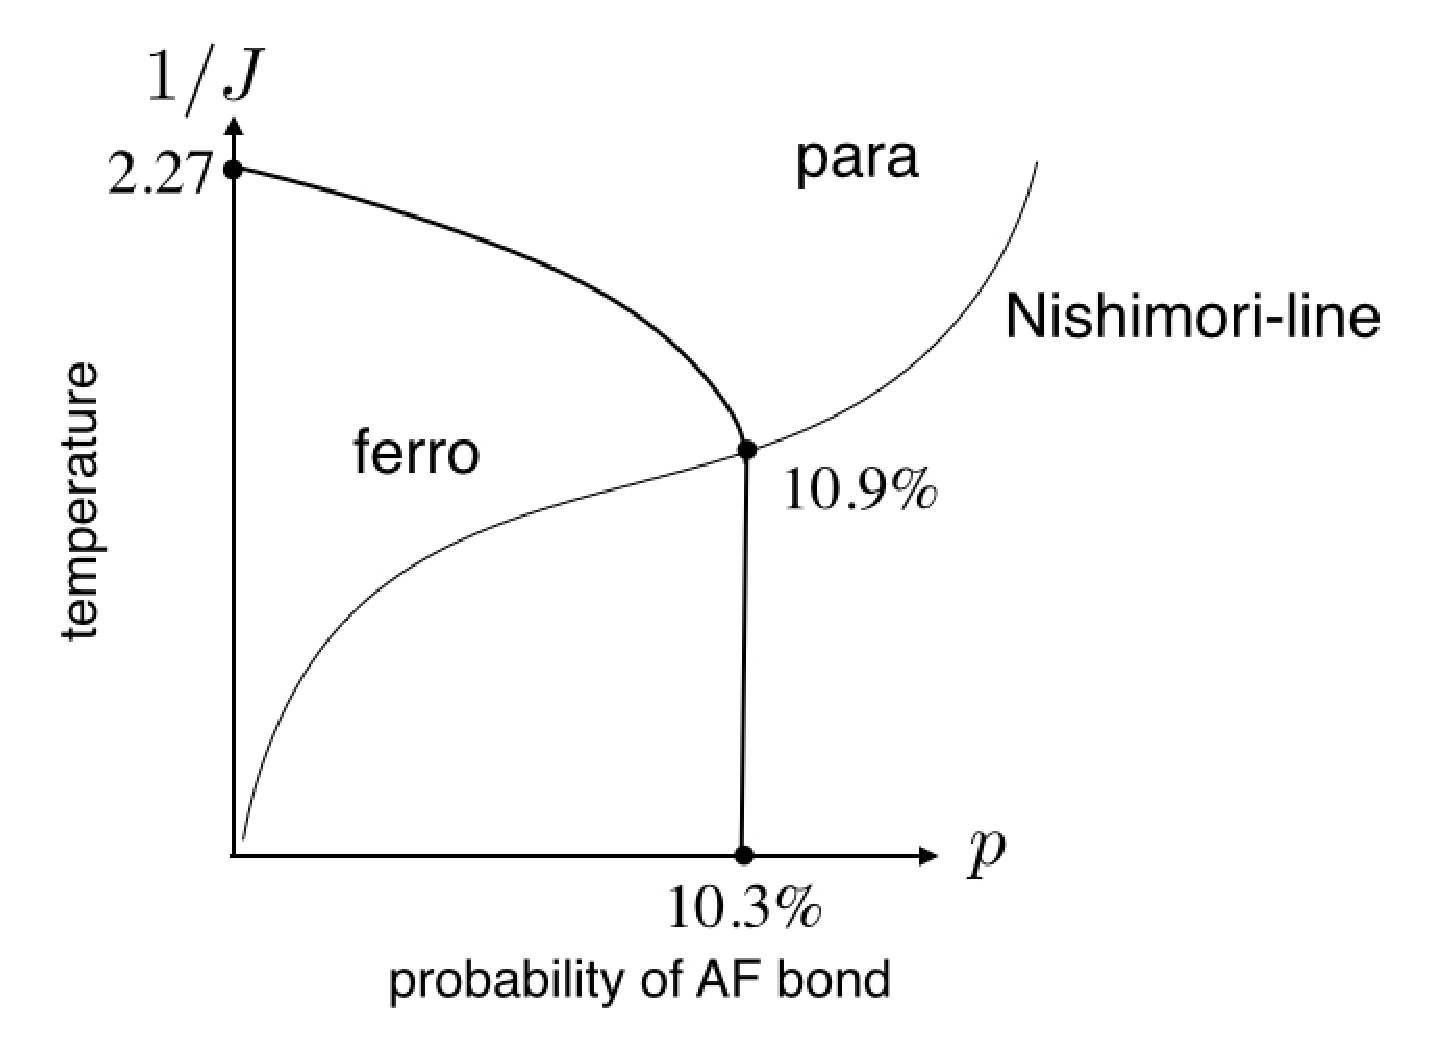
\includegraphics[width=90mm]{fig65.eps}
%
% If not, use
%\picplace{5cm}{2cm} % Give the correct figure height and width in cm
%
\caption{A phase diagram of RBIM with respect to the coupling strength $J=(1/2)\ln [p/(1-p)]$ and the probability of anti-ferromagnetic interaction $p'$.
The probability $p$ in $j$ corresponds to the parameter in the posterior probability. 
When $p=p'$, called the Nishimori line\index{Nishimori line}, an optimal decoding is achieved. }
\label{fig65}       % Give a unique label
\end{figure}
As mentioned before, optimal decoding is achieved with $p=p'$, 
i.e., $e^{-J}=\sqrt{p'/(1-p')}$, 
which is called the Nishimori line~\cite{Nishimori81}.
The critical point on the Nishimori line, which is called a multi-critical point, has been numerically calculated to be $10.94\pm 0.02\%$ by Honecker {\it et al.} and 
Merz {\it et al.}~\cite{Reis99,Honecker01,Merz02}.
The optimal threshold value of the surface code is good in the following sense:
The existence of CSS codes with asymptotic rate $R\equiv k/n$ is guaranteed if
\begin{eqnarray}
R=1 - 2 H_2 (p),
\end{eqnarray}
by the quantum Gilbert-Varshamov bound\index{quantum Gilbert-Varshamov bound} under independent $X$ and $Z$ errors with probability $p$~\cite{CalderbankShor}.
The rate becomes zero with $p=11.00\%$.
The optimal threshold of the surface code, which consists only of local stabilizer generators, achieves a value very close to this.
Indeed, Nishimori conjectured that the multi-critical point of the RBIM is determined by 
\begin{eqnarray}
 H_2 (p)= 1/2,
\end{eqnarray}
arguing from the self-duality in RBIM with a replica method~\cite{NishimoriNemoto,NishimoriConj,KramersWannier} (if the reader is interested this derivation, please see a review in Ref.~\cite{OhzekiKindaiBook}).
Ohzeki has evaluated the multi-critical point precisely to be $10.92\%$ by using a real-space renormalization~\cite{Ohzeki09}, which is in a good agreement with the numerical result~\cite{Hasenbusch08}.

The minimum distance decoding with MWPM is achieved in the limit $p \rightarrow 0$, which is the low temperature limit $J \rightarrow \infty$ where the entropic effect is suppressed.
The threshold of MWPM corresponds to the critical point at zero temperature~\cite{Barahona}, which has been investigated numerically and determined to be $10.4\pm 0.1$ by Kawashima {\it et al.}~\cite{Kawashima,Wang,Dennis}.


\begin{table}[htdp]
\caption{The correspondence among 
random-bond Ising model, $\mathbf{Z}_2$ chain complex and stabilizer codes.}
\begin{center}
\begin{tabular}{c|c|c}
\hline
\hline
RBIM & stabilizer code & chain complex 
\\
\hline
dual lattice & $Z$ error correction & primal lattice
\\
primal lattice & $X$ error correction & dual lattice
\\
Ising interactions & qubits & edge $e_l$
\\
gauge spin & $Z$-type stabilizer generators & face $f_m$
\\
gauge spin & $X$-type stabilizer generators & vertex $v_k$ (dual face $\bar f_k$)
\\
domain wall & logical $X$ and $Z$ operators & nontrivial cycles $c_1$ and $\bar c_1$
\\
anti-ferromagnetic interactions & $X$ and $Z$ errors & 1-chains $c_1$ and $\bar c_1$
\\
frustration & $X$ and $Z$ error syndromes & $\partial c_1$ and $\partial \bar c_1$
\\
\hline \hline
\end{tabular}
\end{center}
\label{tab:ChainStabCode2}
\end{table}%



\section{Other topological codes}
\begin{figure}[t]
\centering
%\sidecaption
% Use the relevant command for your figure-insertion program
% to insert the figure file.
% For example, with the option graphics use
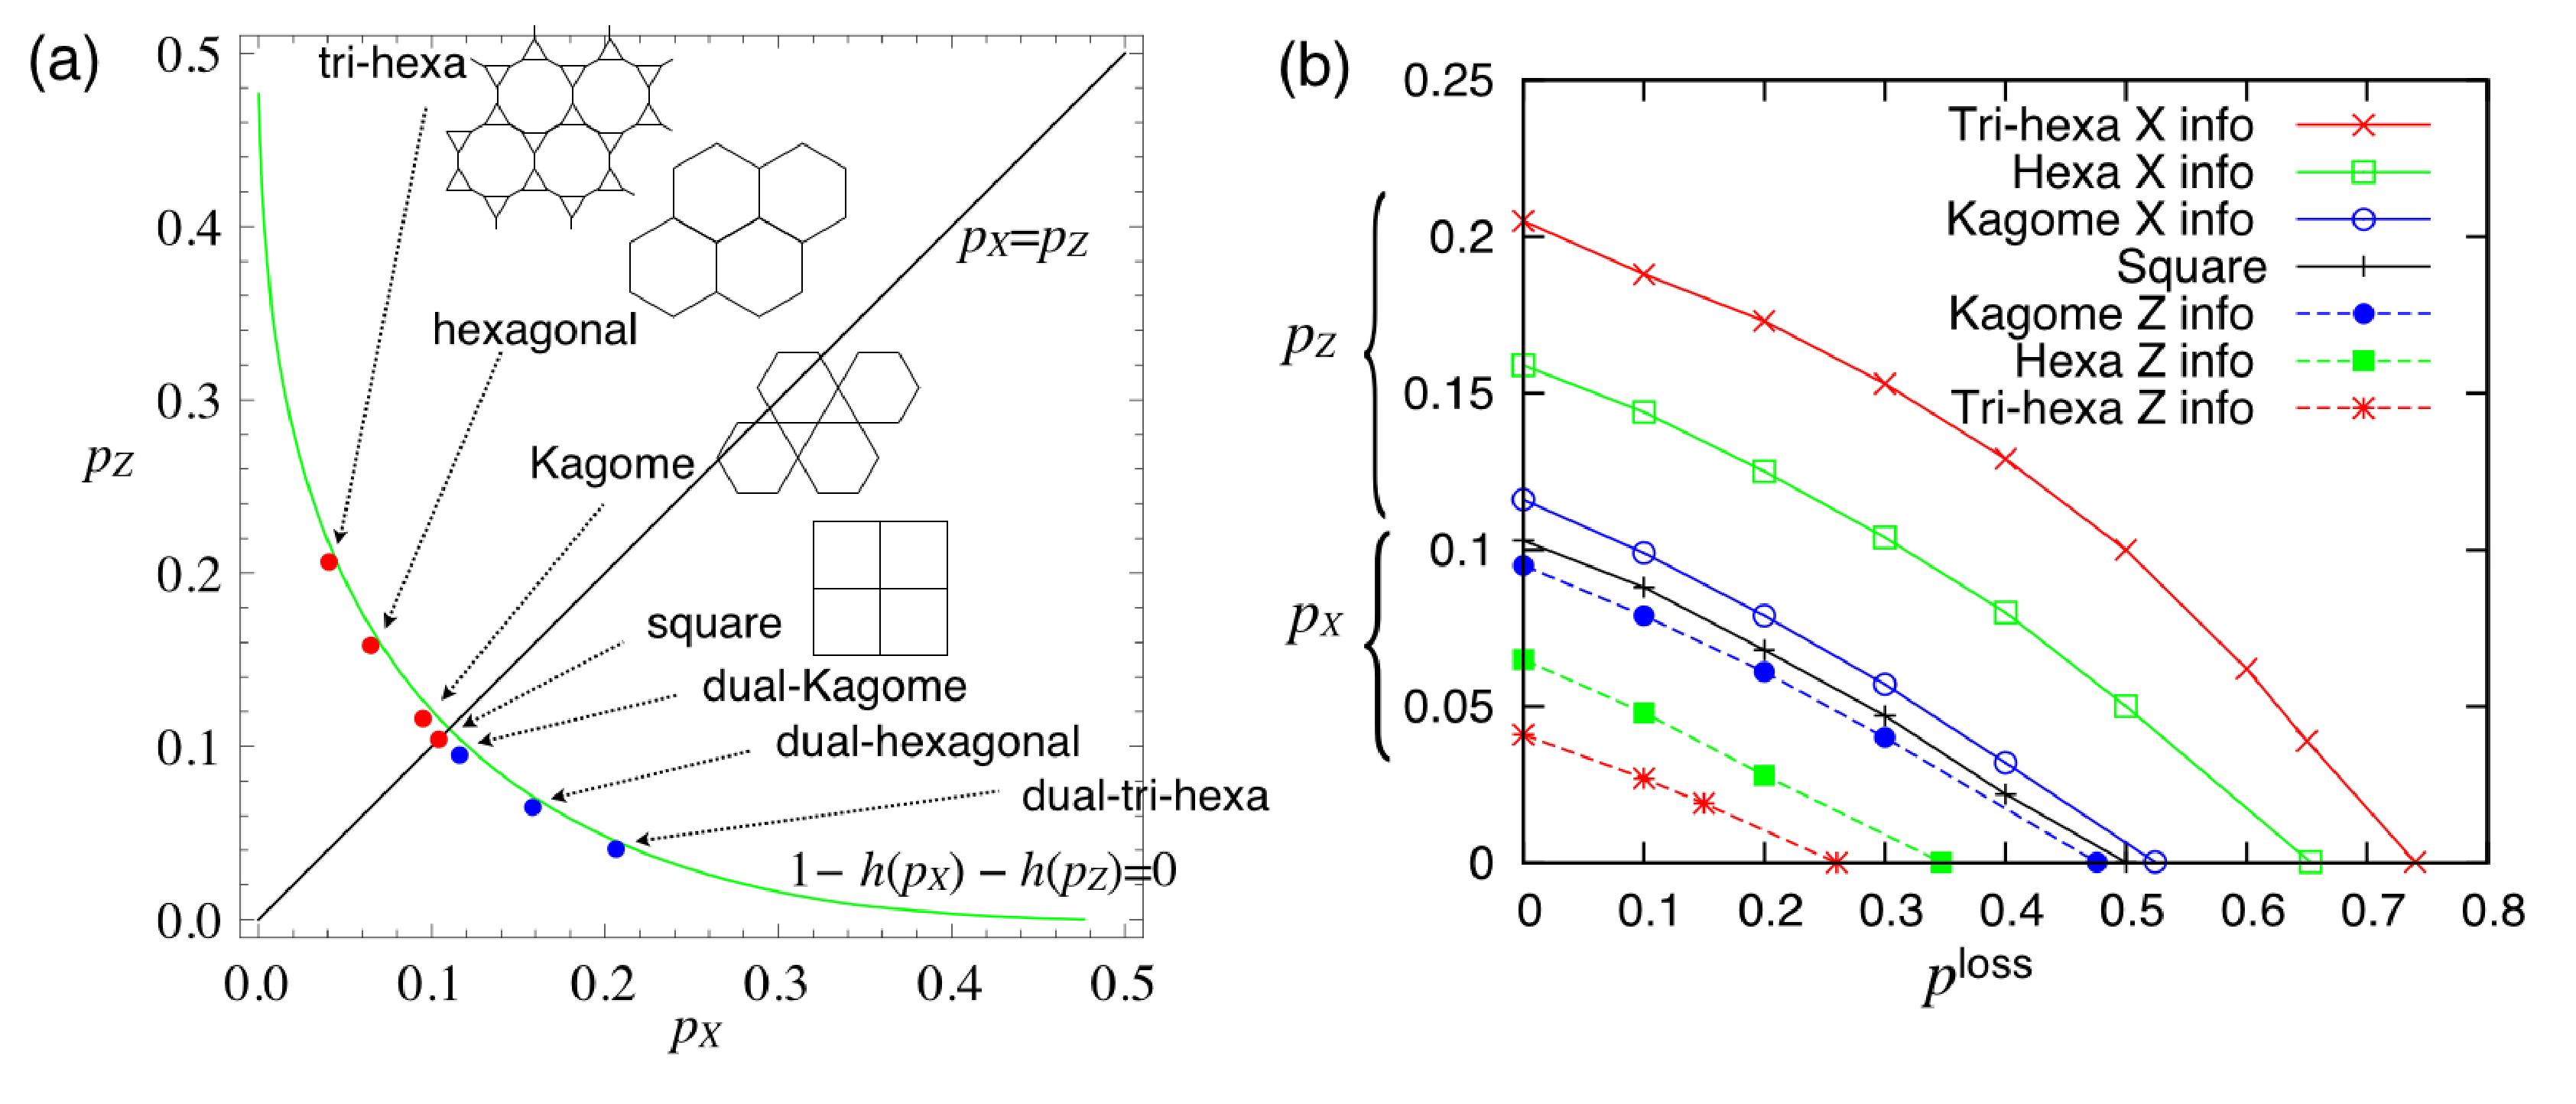
\includegraphics[width=150mm]{fig72.eps}
%
% If not, use
%\picplace{5cm}{2cm} % Give the correct figure height and width in cm
%
\caption{(a) The thresholds $(p_x,p_z)$ of the surface codes on square, Kagome, hexagonal, and triangle-hexagonal lattices, as well as their duals. 
The curve is the quantum Gilbert-Varshamov bound hitting zero asymptotic rate under a bit and phase flip channel with probabilities $p_x$ and $p_z$, respectively.
(b) The trade-off curves between qubit loss rate $p^{\rm loss}$ and unheralded error rates $p_x$ and $p_z$ are shown for square, Kagome, hexagonal, and triangle-hexagonal lattices. 
If the loss and error rates are below these curves, the logical information is protected. }
\label{fig72}       % Give a unique label
\end{figure}

The surface codes have been also studied on general lattice tillings, such as, triangle, hexagonal, and random lattices~\cite{Ohzeki09,Roth,FujiiTokunaga12,OhzekiFujii,Al-Shimary,Kay14}.
Suppose a surface code is defined on a lattice $G=(V,E,F)$.
As seen in the previous section, the $X$ error correction is mapped into a RBIM on a lattice $G=(V,E)$.
On the other hand, the $Z$ error correction is mapped into a RBIM on its dual lattice $\bar G=(\bar V, \bar E)$.
The mutual duality relation\index{mutual duality relation}~\cite{NishimoriNemoto} between $G$ and $\bar G$ allows us to predict the relation between the optimal threshold values 
for $X$ and $Z$ errors:
\begin{eqnarray}
H(p_x)+H(p_z)=1,
\label{eq:mutual_duality}
\end{eqnarray}
where $p_x$ and $p_z$ are the $X$ and $Z$ error probabilities, respectively.
This equality is the same as the quantum Gilbert-Varshamov bound evaluated for the independent $X$ and $Z$ errors with probabilities $p_x$ and $p_z$, respectively.
The precise locations of the optimal thresholds for regular lattices have been investigated by Ohzeki using a real-space renormalization technique~\cite{Ohzeki09}.
The thresholds have been investigated using the MWPM algorithm by Fujii {\it et al.}~\cite{FujiiTokunaga12}.
The thresholds with MWPM (i.e., the critical points of RBIMs at zero temperature) even approaches Eq.\ (\ref{eq:mutual_duality}), as shown in Fig.~\ref{fig72}.
These codes with an asymmetry between the $X$ and $Z$ error tolerances would be useful to correct a biased error~\cite{BiasedNoiseNJP}.
In Refs~\cite{Roth,OhzekiFujii}, the asymmetry is continuously controlled by changing a lattice parameter.

\begin{figure}[t]
\centering
%\sidecaption
% Use the relevant command for your figure-insertion program
% to insert the figure file.
% For example, with the option graphics use
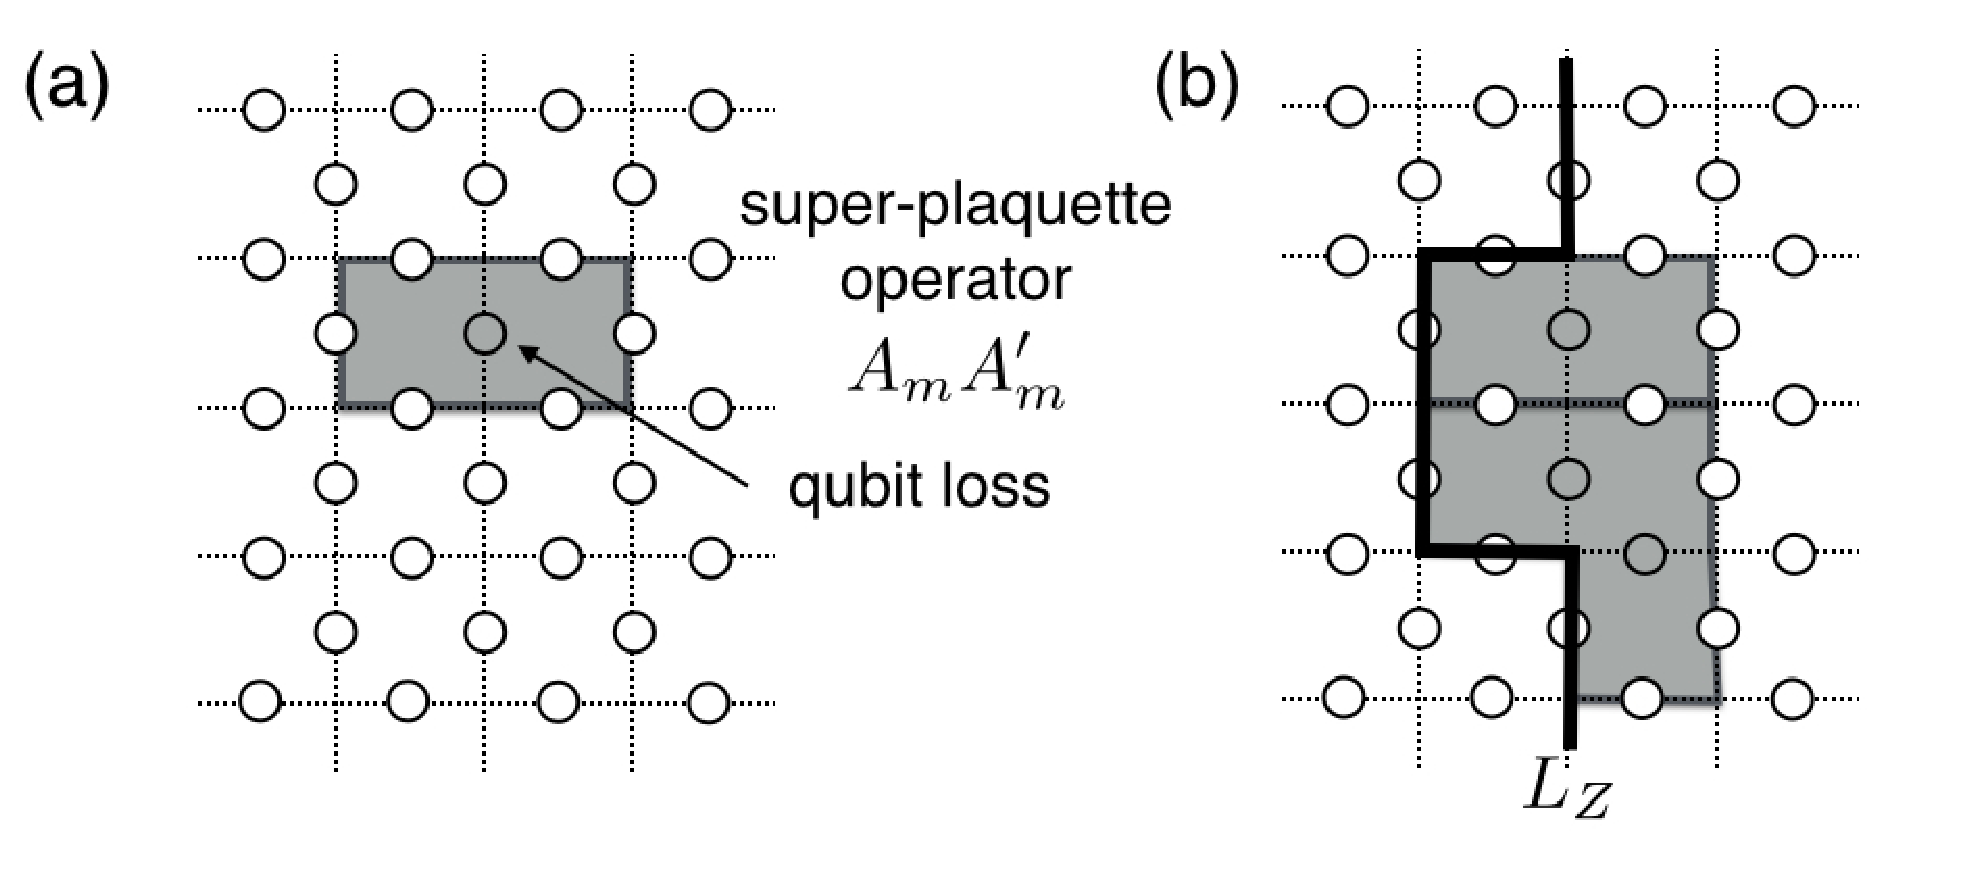
\includegraphics[width=120mm]{fig67.eps}
%
% If not, use
%\picplace{5cm}{2cm} % Give the correct figure height and width in cm
%
\caption{(a) A super-plaquette defined as a product of two plaquette operators. 
The lost qubit is not contained in the super-plaquette operator. 
(b) The logical operator is chosen appropriately by avoiding the lost qubits. 
The lost qubits (bonds) are not percolated, so we can find such a logical operator.}
\label{fig67}       % Give a unique label
\end{figure}
A leakage process or qubit loss is an important source of noise.
Unlike the $X$ and $Z$ errors discussed so far, the qubit loss is detectable (heralded), and hence we can tolerate much more loss rate than for the (undetectable) error rate.
Stace {\it et al.} proposed to cope with the qubit loss on the surface code~\cite{StacePRL,StacePRA}. 
Suppose a qubit is lost on the surface as shown in Fig.~\ref{fig67} (a).
The plaquette operators containing the lost qubit are undetermined. 
However, we can construct a {\it super-plaquette} multiplying two neighboring plaquette so that the super-plaquette does not have the lost qubit.
By using the super-plaquette as a stabilizer generator, we can perform MWPM.
If two super-plaquettes are neighbors, the weight between these super-plaquettes has to be modified appropriately in MWPM, because the plaquettes share two physical qubits and the error probability is effectively doubled.
The logical operator is defined by avoiding the lost qubits.
Unless the lost qubits, which are located on edges, are percolated throughout the lattice, we can find such a logical operator.
Thus, the threshold for qubit loss in the large lattice limit without any (undetected) error is determined by the bond percolation threshold.
The trade-off curves between qubit loss and (unheralded) error rates with MWPM for various lattice tillings are shown in Fig.~\ref{fig72} (b).

On the other hand,
when the error correction problem is mapped into the RBIM,
the qubit loss corresponds to a bond-dilution.
The duality relation in the presence of the bond-dilution on the square lattice is given by~\cite{OhzekiLoss}
\begin{eqnarray}
(1-q)h(p)+q=1/2.
\label{eq:duality_loss}
\end{eqnarray}
From the numerical data in Refs.~\cite{FujiiTokunaga12}, we could expect a more general equality,
\begin{eqnarray}
(1-q_x) h(p_x)+(1-q_z)h(p_z)+q_x+q_z=1,
\label{eq:m_duality_loss}
\end{eqnarray}
where $q_x$ and $q_z$ are the probabilities of the heralded $X$ and $Z$ errors, respectively.
With $p_x=p_z=0$, this is reduced to $q_x+q_z=1$, which corresponds to Kesten's duality relation of the bond percolation thresholds between mutually dual lattices.
With $q_x=q_z=0$, Eq.\ (\ref{eq:m_duality_loss}) is reduced to Eq.\ (\ref{eq:mutual_duality}).
With $q_x=q_z=q$ and $p_z=p_x=p$, Eq.\ (\ref{eq:m_duality_loss}) is reduced to Eq.\ (\ref{eq:duality_loss}).

Another important class of local stabilizer codes is the topological color code\index{topological color code} proposed by Bombin and Martin-Delgado~\cite{Bombin06,Bombin07}.
\begin{figure}[t]
\centering
%\sidecaption
% Use the relevant command for your figure-insertion program
% to insert the figure file.
% For example, with the option graphics use
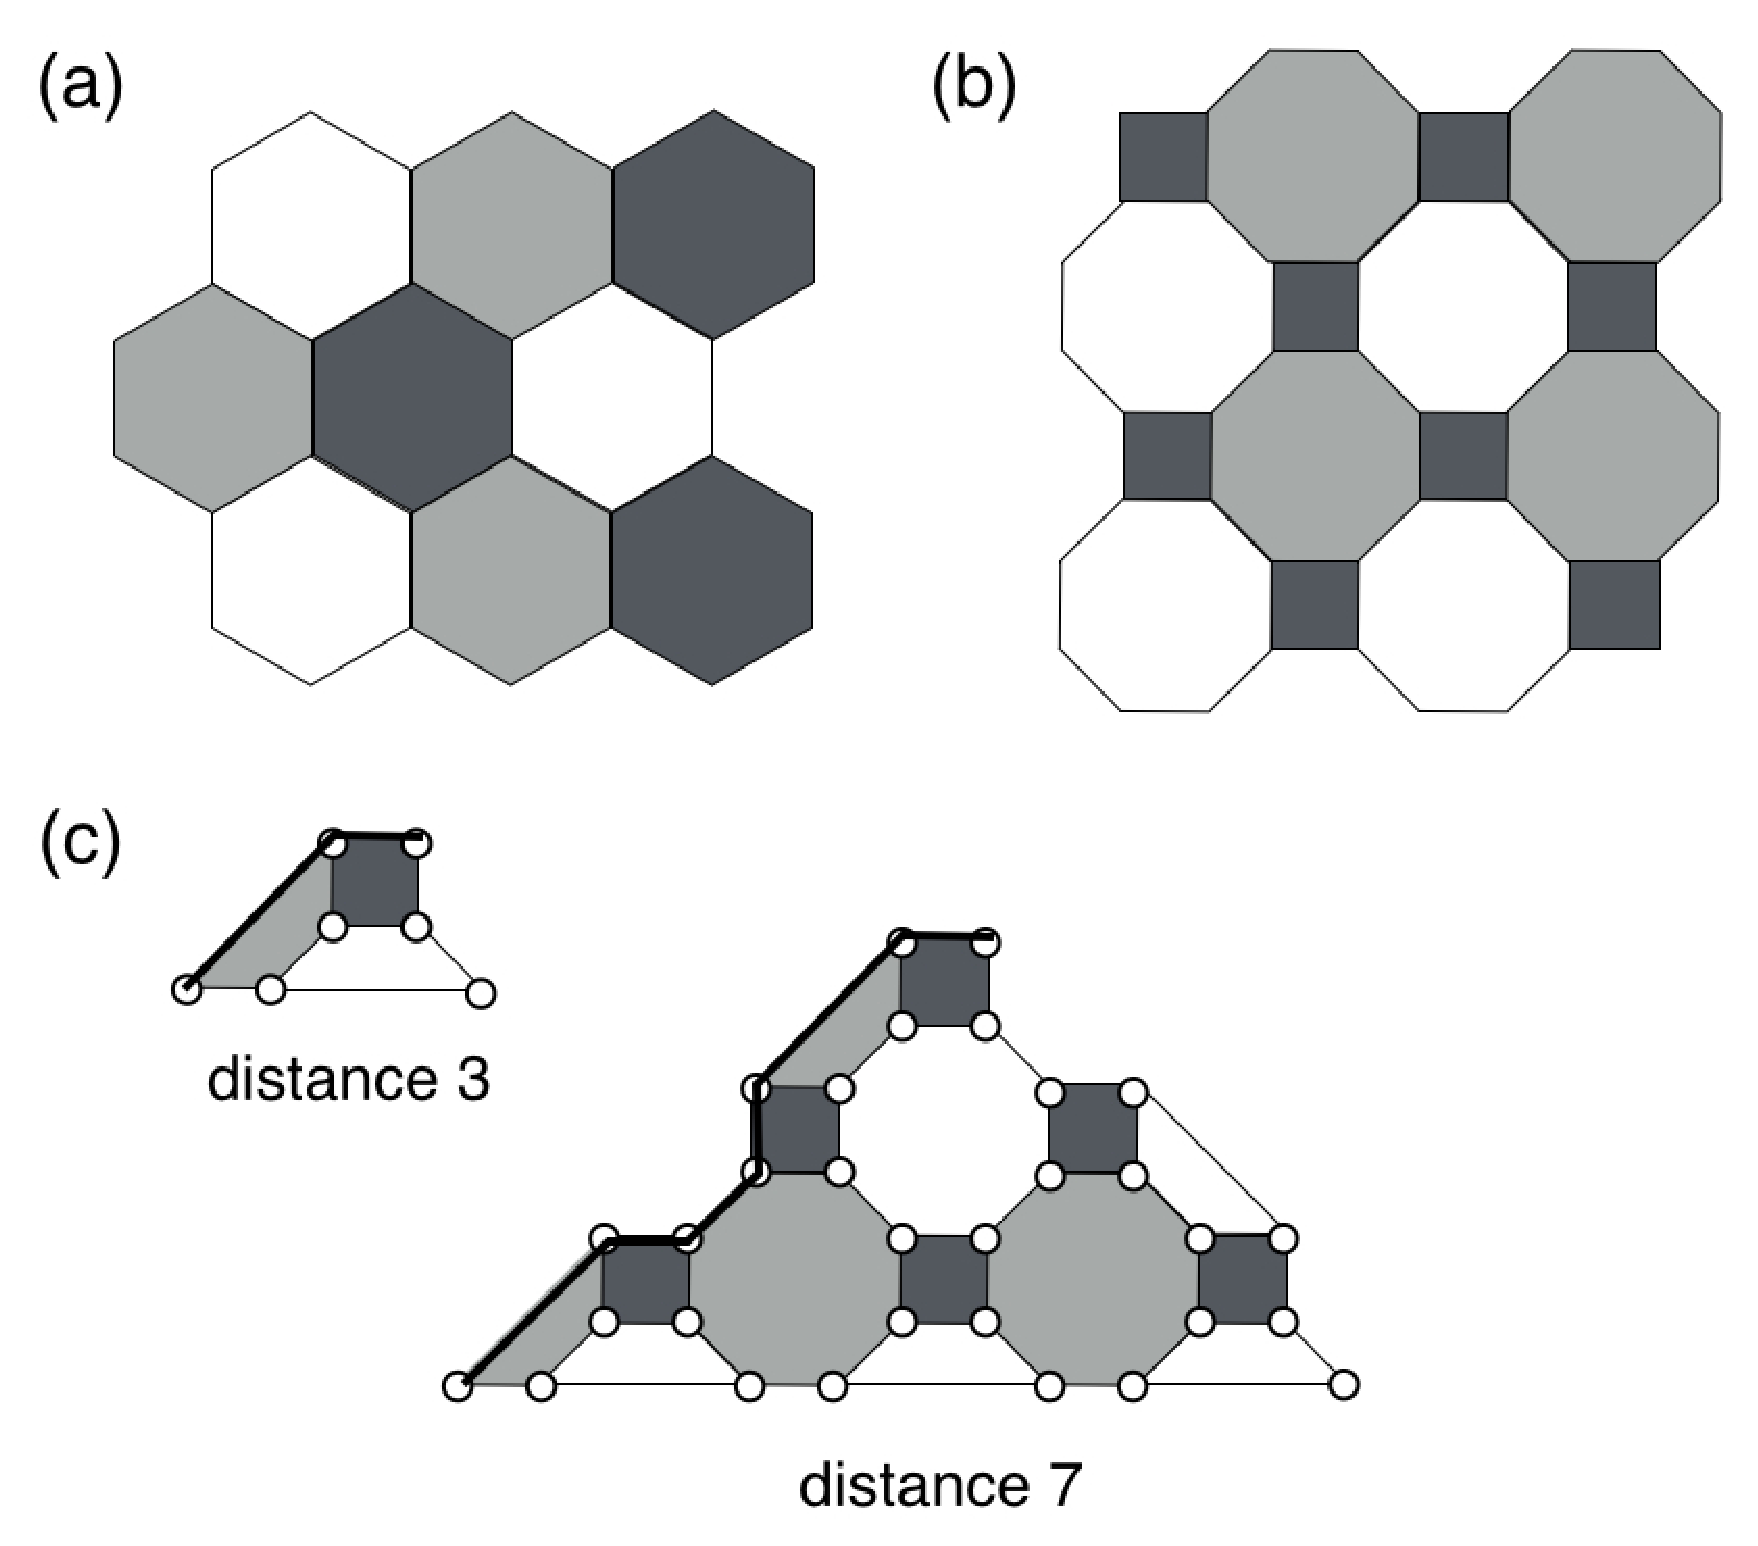
\includegraphics[width=100mm]{fig69.eps}
%
% If not, use
%\picplace{5cm}{2cm} % Give the correct figure height and width in cm
%
\caption{(a) and (b) Trivalent lattices that can be colored with three distinct colors. 
(c) Color codes defined on (4.8.8) lattices with a triangle open boundary condition. 
The logical operators are shown by solid lines. 
Any string at the boundaries can be employed as a logical operator.}
\label{fig69}       % Give a unique label
\end{figure}
The topological color codes are defined on trivalent graphs with faces that can be colored with three colors, such as
hexagonal (6.6.6) and (4.8.8) lattices, as shown in Fig.~\ref{fig68} (a) and (b), respectively.
A qubit is defined on each vertex $v$ and stabilizer generators are defined on each face $f$:
\begin{eqnarray}
B^{x}= \prod _{v \in f} X_v , \;\;\;B^{z}= \prod _{v \in f} Z_v.
\label{eq:color_stab}
\end{eqnarray}
Specifically, the color code on a (4.8.8) lattice, shown in Fig.~\ref{fig69} (c), allows all single-qubit Clifford gates transversally.
The distance-3 topological color code on the (4.8.8) lattice is equivalent to Steane's 7-qubit code~\cite{Steane96}.
The extension to a 3D lattice also enables a transversal non-Clifford gate on the code space~\cite{Bombin07}, whose distance-3 version corresponds to the Reed-Mullar 15-qubit code~\cite{Magic}.

The topological color codes are also described by a $Z_2$ chain complex on hyper-graphs~\cite{Delfosse14}.
Consider a trivalent graph $G=(V,E)$, on which a topological color code is defined.
We define a hyper-graph $\mathcal{G}=(\mathcal{V}, \mathcal{E},\mathcal{F})$ consisting of the sets of hyper-vertices $\mathcal{V}$, hyper-edges $\mathcal{E}$, and hyper-faces $\mathcal{F}$ as follows (see Fig.~\ref{fig68}):
\begin{figure}[t]
\centering
%\sidecaption
% Use the relevant command for your figure-insertion program
% to insert the figure file.
% For example, with the option graphics use
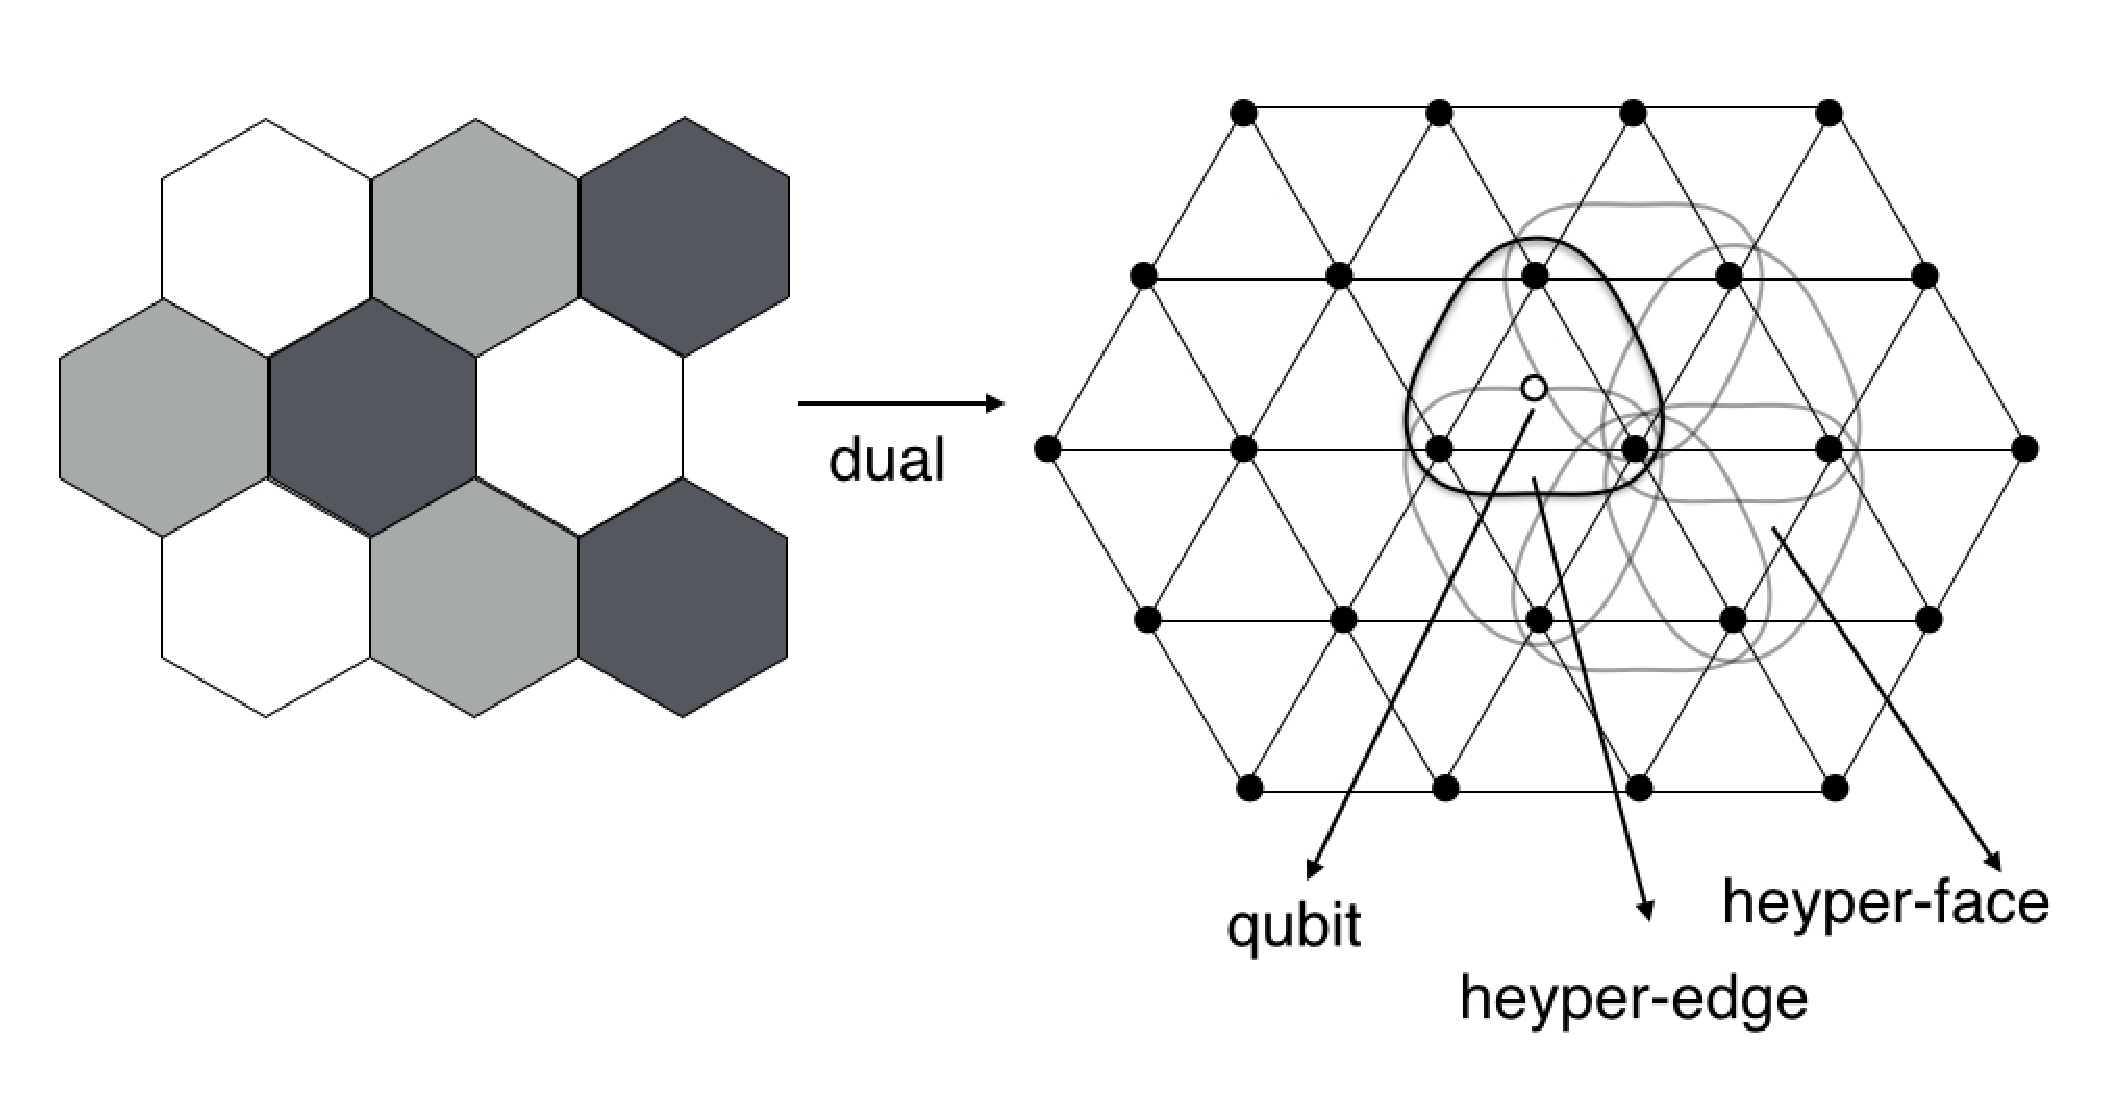
\includegraphics[width=120mm]{fig68.eps}
%
% If not, use
%\picplace{5cm}{2cm} % Give the correct figure height and width in cm
%
\caption{(left) A hexagonal lattice with three-coloring. 
(right) A triangular lattice, the dual of the hexagonal lattice. 
A hyper-graph is defined on a triangular lattice. The color code on the hexagonal lattice corresponds to a surface code defined on the hyper-graph.}
\label{fig68}       % Give a unique label
\end{figure}
The hyper-vertices $\mathcal{V}$ are vertices $\bar V$ of the dual graph $\bar G$.
A hyper-edge $ \tilde{e} \in \mathcal{E}$ is defined as a triplet of (hyper-)vertices $\bar v \in \bar V$ on a face $\bar f$ of the dual graph $\bar G$.
A hyper-face $\tilde f \in \mathcal{F}$ is defined as a set of hyper-edges $\tilde{e}$ that are incident to the vertex $\bar v$ of the dual graph $\bar G$.
As defined in Sec.~\ref{sec:chain_complex}, we can define both $\mathbf{Z}_2$ valued vector spaces and Abelian groups $C_{1,2,3}$ with the hyper-graph elements as their bases.
Because the hyper-edge and hyper-face are defined as sets of hyper-vertices and hyper-edges, respectively, we can define boundary maps $\partial _i : C_i \rightarrow C_{i-1}$ 
naturally by such sets.
The plaquette and star stabilizer generators of the surface code defined on such a hyper-graph are as follows:
\begin{eqnarray} 
A_{m} = \prod _{\tilde e \in \partial \tilde f} Z_{\tilde e},
\;\;\;
B_k = \prod _{\tilde e \in \delta \tilde v} X_{\tilde e}.
\end{eqnarray}
This definition is equivalent to the previous definition, Eq.\ (\ref{eq:color_stab}).
In Ref.~\cite{Delfosse14}, the authors defined the projections from the $\mathbf{Z}_2$ chain complex on the hyper-graph into chain complexes on a dual graph $\bar G$.
Specifically, a certain subset of vertices is removed in each projection.
This procedure corresponds to the removal of stabilizer generators colored by one of the three colors.
This allows us to utilize MWPM to decode the topological color codes efficiently on the projected surface codes~\cite{Delfosse14}.

The decoding problem of topological color codes is mapped into random three-body Ising models using the mapping between quantum error correction and spin glass models. 
This can be understood as follows. 
For each face center a gauge spin valuable 
is located associated with each stabilizer generator;
three gauge spin valuables (stabilizer generators) 
that share the same qubit (vertex)
interact with each other.
The locations of the optimal thresholds have also been investigated via the spin glass theory and Monte Carlo simulations~\cite{OhzekiColor,BombinOhzeki}.


\section{Connection to topological order in condensed matter physics}
Topological order\index{topological order, topological ordered system} is an exotic quantum phase of matter, which cannot be characterized by the Landau-Ginzburg theory of symmetry breaking, in which an ordered phase can be characterized by local order parameters.
The ground state of a topologically ordered system is degenerate, but its degeneracy cannot be destroyed by any local perturbation. 
Thus, no local order parameter can succeed to capture the topologically ordered phase.
Understanding the nature of topological order is one of the most important goals of modern condensed matter physics.
Moreover, the ground state of a topologically ordered system is, by definition, robust against any local perturbations, and hence it is also useful for storing quantum information.
There is a beautiful correspondence between topological quantum codes and topologically ordered systems, which provides a promising way to understand condensed matter physics
via quantum information.

Let us first consider the bit-flip code defined in Sec.~\ref{sec:bit-flip}.
The Hamiltonian, which we call a stabilizer Hamiltonian\index{stabilizer Hamiltonian}, is defined as follows:
\begin{eqnarray}
H_{\rm Ising} = - J \sum _k A_k = -J \sum _{i=1}^{n-1} Z_iZ_{i+1}.
\label{eq:Hami_Ising}
\end{eqnarray}
Here, the summation is taken over all stabilizer generators, but one stabilizer operator, which is not independent, is removed.
The Hamiltonian Eq.\ (\ref{eq:Hami_Ising}) corresponds to the Ising model in 1D with an open boundary condition.
By its construction, the Hamiltonian is diagonalizable, and the stabilizer state becomes the ground state.
The bit-flip code has a 2D stabilizer subspace spanned by $\{ |00...0\rangle, |11...1\rangle\}$.
This means that the ground state is degenerate.
The bit-flip errors occurring on the code space excite the ground state to an excited state.
Thus, the states in the orthogonal subspaces of the bit-flip code correspond to excited states.

To address topological order, let us consider the robustness of the ground state against perturbations from transversal fields $h_x\sum _i X_i$.
By using standard perturbation theory~\cite{Kato}, we can show that the degeneracy of the ground states is not lifted up to the $(n-1)$th order of perturbation.
This happens because the code distance of the $n$-qubit bit flip code against $X$ errors is $n$, and any $X$ errors of weight up to $n-1$ map the code state into an orthogonal space.
Accordingly, the ground state degeneracy is robust against the transversal fields.

On the other hand, longitudinal fields $h_z \sum _{i}Z_i$ spoil the ground state degeneracy in the large $n$ limit, even if $h_z$ is small. 
More precisely, the energy between $|00..0\rangle$ and $|11..1\rangle$ is shifted by $n h_z$.
Thus, a superposition $\alpha |00..0\rangle + \beta |11..1\rangle$ in the ground subspace is easily destroyed by the longitudinal fields.
In this sense, the stabilizer Hamiltonian constructed by the bit-flip code is not topologically ordered.
However, if any perturbation with respect to the longitudinal fields is prohibited due to some symmetry of nature, the ground state degeneracy is robust under that symmetry.
This type of robustness of ground-state degeneracies is called {\it symmetry protected topological order}\index{symmetry protected topological order}~\cite{SymmetGuWen,SymmetPollMann}.
(Note that in this case the ground-state degeneracy is 
not related to the geometrical property of the underlying manifold
in contrast to the genuine topological order in 2D.)

The symmetry prohibiting the longitudinal fields seems to be somewhat artificial.
We can, however, impose the symmetry by transforming the Ising Hamiltonian to a free-fermion model using the following Jordan-Wigner transformation\index{Jordan-Wigner transformation}~\cite{JWtrans}:
\begin{eqnarray}
a_{2i-1} =\prod _{k=1}^{i-1} X_k Z_i,
\\
a_{2i} = \prod _{k=1}^{i-1} X_k Y_i.
\end{eqnarray}
The operators, called Majorana fermion\index{Majorana fermion} operators, are hermitian $a_k= a_k^{\dag}$ and satisfy the fermion commutation relation 
$\{ a_{k}, a_{k'} \} = \delta _{k,k'}I$.
The Ising stabilizer Hamiltonian is reformulated in terms of $a_k$:
\begin{eqnarray}
H_{\rm Isng}= -J \sum_{i=1}^{n-1} (-i) a_{2i} a_{2i+1}.
\end{eqnarray}
The logical operators acting on the degenerated ground states are given by
\begin{eqnarray}
L_Z=a_1=Z_1, \;\; L_Y=a_{1} a_{2n}= Y_1 \left(\prod _{k=2}^{n-1}X_k \right) Y_n.
\end{eqnarray}
The degree of freedom in the degenerated ground states is called the Majorana zero mode or the unpaired Majorana fermion~\cite{KitaevMajorana}.
If the parity of the number of fermions is preserved, the fermion operators would appear with a quadratic form $a_k a_k'$.
Under such a symmetry, there is no perturbation that lifts the ground state degeneracy. 
Thus, the ground state of the unpaired Majorana fermion is symmetry protected.

\begin{figure}[t]
\centering
%\sidecaption
% Use the relevant command for your figure-insertion program
% to insert the figure file.
% For example, with the option graphics use
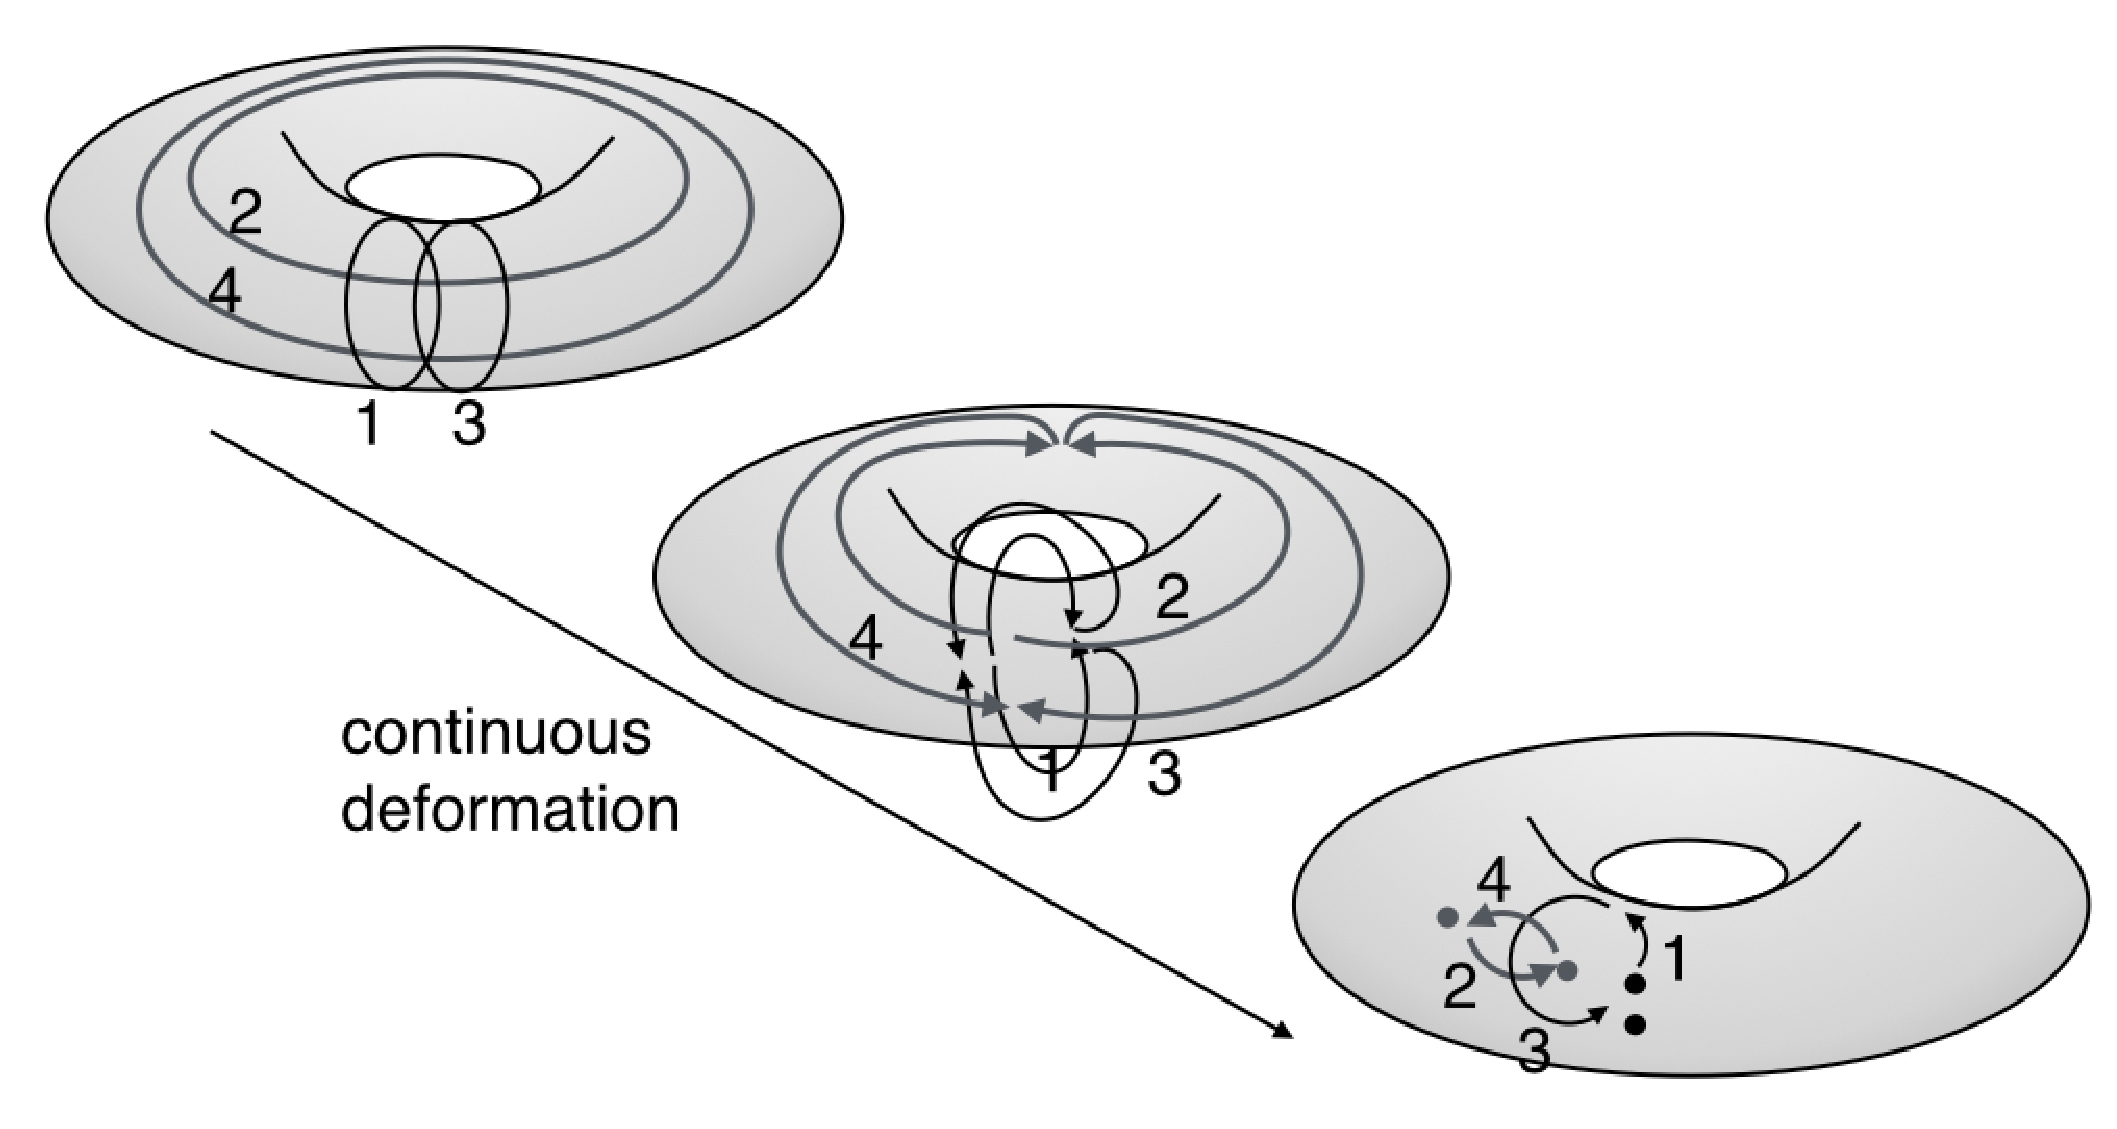
\includegraphics[width=110mm]{fig70.eps}
%
% If not, use
%\picplace{5cm}{2cm} % Give the correct figure height and width in cm
%
\caption{(left top) (1) A pair of $X$-type excitations are created, moved around the torus, and annihilated. 
(2) A pair of $Z$-type excitations are created, moved around the torus, and annihilated. 
(3) Do the process (1) again. 
(4) Do the process (2) again. 
(middle) The creation, movement, and annihilation process is continuously deformed. 
(right bottom) A braiding operation of an $X$-type excitation around a $Z$-type excitation.}
\label{fig70}       % Give a unique label
\end{figure}
Next, we will provide a genuine topologically ordered system based on the surface code (Kitaev's toric code).
The stabilizer Hamiltonian, the so-called Kitaev's toric code Hamiltonian \index{Kitaev's toric code Hamiltonian}~\cite{Kitaev97}, is given as a summation of all plaquette and star operators:
\begin{eqnarray}
H_{\rm Kitaev} = -J \sum _{m}A_m - J \sum _{k} B_k.
\end{eqnarray}
The ground state has a fourfold degeneracy corresponding to the code space.
Errors on the code state correspond to excitations.
Specifically, there are two types of excitations, corresponding to the $Z$ error $Z( c_1)$ and $X$ error $X(c_1)$.
Excitations appear at the boundaries of the error chains $\partial c_1$ and $\partial \bar c_1$, because the local energy changed from $-J$ to $+J$ there.
Such excitations, i.e., at the end points of the error chains, are always created as pairs, can be viewed as a pair creation process on the ground state.

Suppose these two types of the excitations were created on the system and moved as shown in Fig.~\ref{fig70} (left top).
This process can be described by
\begin{eqnarray}
Z(c_1^{(2)})X(\bar c_1^{(2)})Z(c_1^{(1)})X(\bar c_1^{(1)}) |\Psi \rangle =- |\Psi \rangle.
\label{eq:topo_braid}
\end{eqnarray}
On the other hand, by continuously changing the trajectory of the particles, as shown in Fig.~\ref{fig70}, this process can also be regarded as a braiding process of an $X$-type excitation around a $Z$-type excitation.
After the braiding operations, a phase factor is applied to the state
as shown in the r.h.s. of Eq. (\ref{eq:topo_braid}).
Thus, the excitations are neither bosonic nor fermionic, which are invariant under the braiding operation, i.e., the swapping operation twice.
In this sense, the excitations on the surface code are referred to as anyons.
Specifically, since the phase factors is $\mathbf{Z}_2$, 
they are called $\mathbf{Z}_2$ Abelian anyons\index{Abelian anyon}.
By using the generalized Pauli operators
on for the qudit,
we can also define $\mathcal{Z}_d$ Kitaev's toric code~\cite{Kitaev},
on which excitations are $\mathcal{Z}_d$ Abelian anyons.
More generally, using a finite group $G$,
we can define a quantum state $|g\rangle$ ($g \in G$)
in a $|G|$-dimensional Hilbert space.
Then we define four types of operators for each $g \in G$:
\begin{eqnarray}
L^g_+ = \sum _{h \in G} |gh \rangle \langle h|,
L^g_- = \sum _{h \in G} |hg^{-1} \rangle \langle h|,
T_+^h= |h\rangle \langle h|,
T_-^h= |h^{-1}\rangle \langle h^{-1}|.
\end{eqnarray}
The non-Abelian Kitaev's toric code model,
which is called the quantum double model~\cite{Kitaev},
is defined as
\begin{eqnarray}
H=-J\sum _{m} A(f_m) -J \sum _{k} B(v_k),
\end{eqnarray}
in terms of
the following plaquette and star operators
\begin{eqnarray}
A(f_m) &=& \sum _{g_1 g_2 g_3 g_4 = I} T_-^{g_1}(e^m_{l_1})T_-^{g_2}(e^m_{l_2})
T_+^{g_3}(e^m_{l_3})T_+^{g_4}(e^m_{l_4})
\\
B(v_k) &=& \frac{1}{|G|}\sum _{g \in G} L_+^{g} (\bar e^k_{l_1})
L_+^{g}(\bar e^k_{l_2}) L_-^{g} (\bar e^k_{l_3}) L_-^{g} (\bar e^k_{l_4})
\end{eqnarray}
where the four edges $e^m_{l_{1,2,3,4}} \in \partial f_m$ 
and $\bar e^k_{l_{1,2,3,4}} \in 
\delta v_k = \partial \bar f _k$
are labeled clock wise.
The quantum double model
supports non-Abelian anyonic excitations~\cite{Kitaev,Pachos2012},
which allows us to implement universal quantum computation 
solely by braiding them.

Let us return to the $\mathbb{Z}_2$ Kitaev's toric code Hamiltonian.
The code distance of the surface code on the $n\times n$ torus is $n$.
Thus, neither $X$-type (transverse) nor $Z$-type (longitudinal) fields can lift the ground state degeneracy up to the $(n-1)$th order of perturbation.
More generally, no local perturbation can lift the ground state degeneracy in the large $n$ limit.
Thus, the ground state of the Kitaev's toric code Hamiltonian is topologically ordered.
For any properly defined stabilizer code, we can define a stabilizer Hamiltonian, whose ground state is topologically ordered.
However, in condensed matter physics, the local interactions are of central importance.
Thus, it is natural to restrict the stabilizer generators to be spatially local, i.e., topological stabilizer codes.

Only the nearest-neighbor two-body interactions are attained in physically natural systems.
It has been known that the Kitaev's toric code Hamiltonian 
is obtained as an effective low energy model of 
another model consisting only of two-body nearest-neighbor interactions~\cite{Kitaev06}.
Let us consider the following two-body nearest-neighbor model, called Kitaev's compass model\index{Kitaev's compass model}:
\begin{eqnarray}
H_{\rm comp} = - J_x \sum _{(i,j) \in E_x} X_i X_j  - J_y \sum _{(i,j) \in E_y} Y_i Y_j - J_z \sum _{(i,j) \in E_Z} Z_i Z_j ,
\end{eqnarray}
where $E_x$, $E_y$, and $E_z$ are sets of right-up, left-up, and vertical bonds, respectively, of a hexagonal lattice (see Fig.~\ref{fig71} (left)).
If we take the large $J_z$ limit, each vertical bond favors the two-dimensional subspace spanned by $\{ |00\rangle , |11\rangle\}$, because it is stabilized by $Z_iZ_j$.
Thus, in the large $J_z$ limit, we can derive an effective low energy Hamiltonian, which commutes with the $Z_i Z_j$ interactions, by using perturbation theory:
\begin{eqnarray}
H_{\rm eff} = - \frac{J_x^2 J_y^2}{16|J_z|^3} \sum _{ f} \tilde X_{e_1^{f}} \tilde X_{e_2^f} \tilde Y_{e_3^f} \tilde Y_{e_4^f} - J_Z \sum _{e \in E_Z} \tilde Z_{e},
\end{eqnarray}
where $\tilde A_e = A_i A_j$ with $e=(i,j)$ and $A=X,Y,Z$, depending on $e \in E_x, E_y , E_z$.
The edges $\{ e_i^f\}$ are left-up and right-up edges on a hexagonal face $f$ and the summation $\sum_f$ is taken over all faces.
\begin{figure}[t]
\centering
%\sidecaption
% Use the relevant command for your figure-insertion program
% to insert the figure file.
% For example, with the option graphics use
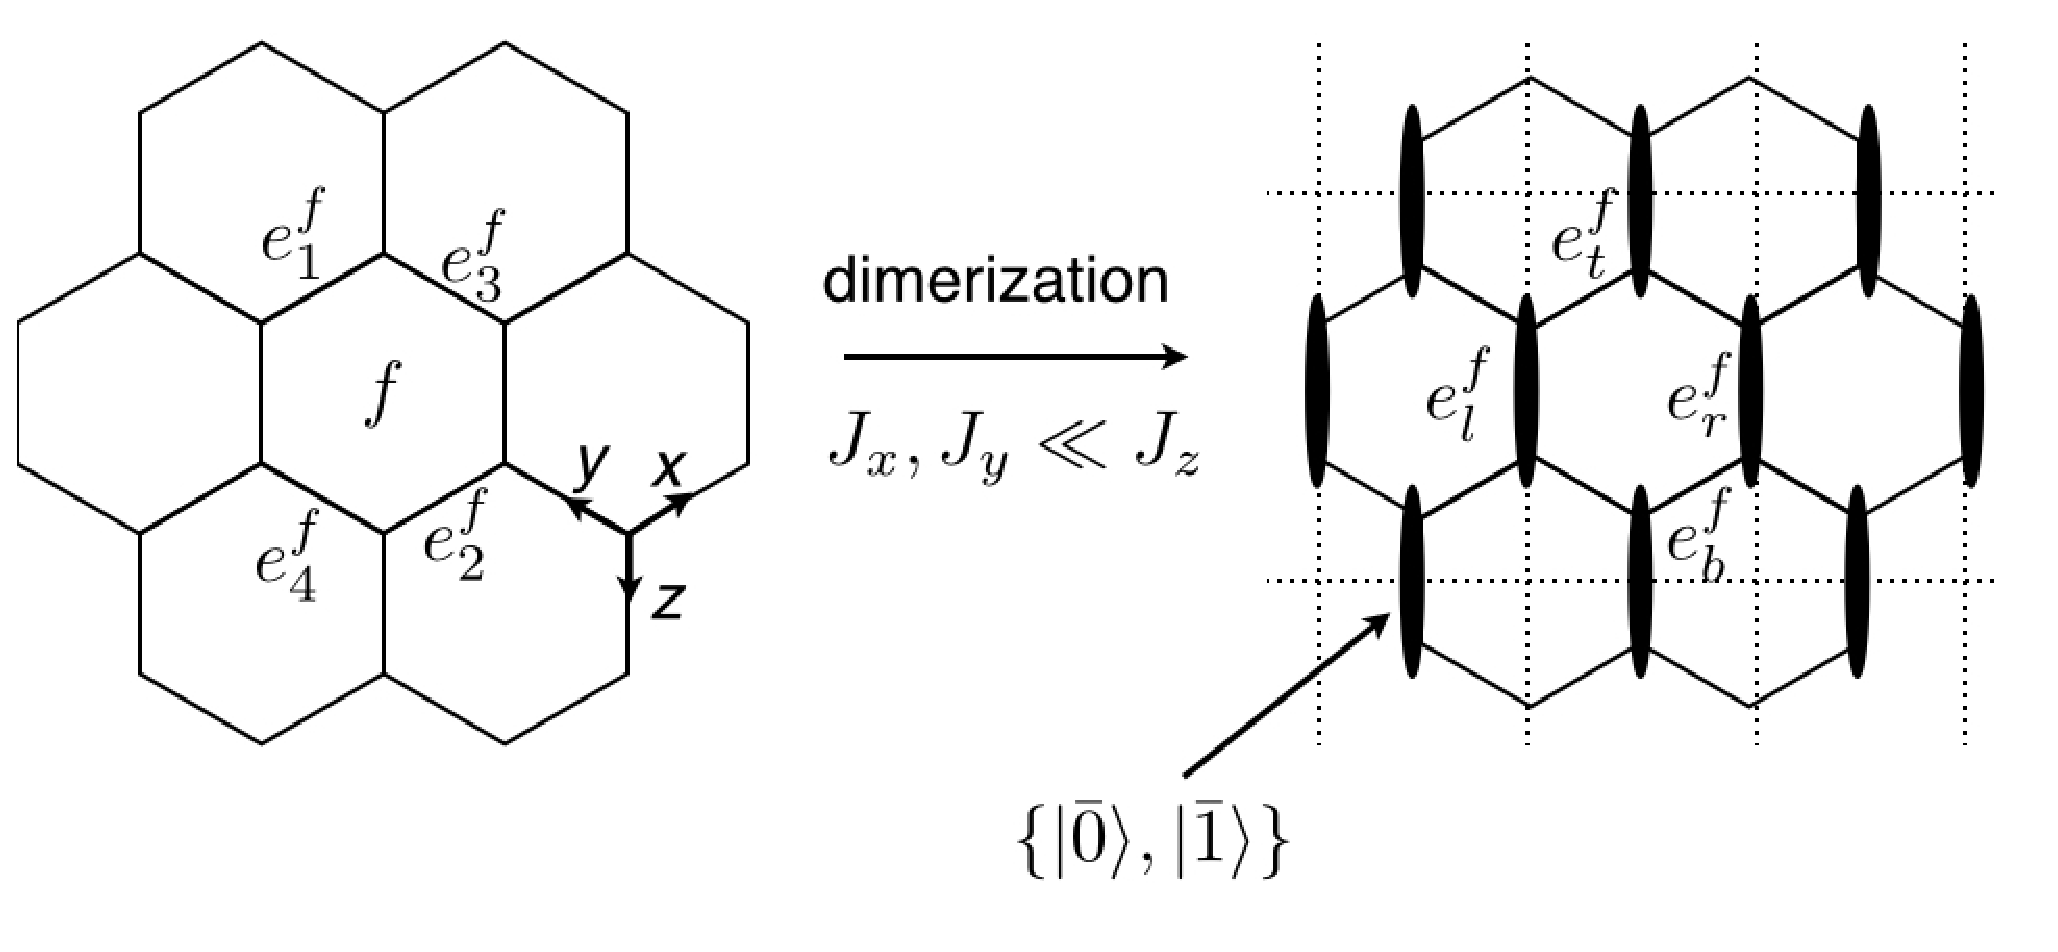
\includegraphics[width=120mm]{fig71.eps}
%
% If not, use
%\picplace{5cm}{2cm} % Give the correct figure height and width in cm
%
\caption{A hexagonal lattice on which Kitaev's compass model is defined.
In the large $J_z$ limit, the two spins on each vertical edge are confined into a 2D subspace forming a dimmer.
The dimmer is located on each edge of a square lattice shown by the dotted lines.}
\label{fig71}       % Give a unique label
\end{figure}

Let us define a qubit $\{ |\bar 0 \rangle =|00\rangle , |\bar 1\rangle =|11\rangle \}$ for each dimerized edge and Pauli operators $\bar X= XX$ or $=\bar YY$ and 
$\bar Z= Z \otimes I$ or $=I \otimes Z$.
Now a qubit is assigned to each edge of a square lattice, which is an vertical edge in the hexagonal lattice as shown in Fig.~\ref{fig71} (right).
Using this definition, the effective Hamiltonian can be reformulated as
\begin{eqnarray}
\bar H_{\rm eff} = - \frac{J_x^2 J_y^2}{16|J_z|^3} \sum _{f} \bar X _{e_l^f} \bar X_{e_r^f} \bar Z_{e_t^f} \bar Z_{e_b^f},
\end{eqnarray}
where $\{ e_l^f, e_r^f, e_t^f, e_b^f\}$ are the left, right, top, and bottom edges, respectively, on a square face $f$.
If we apply the Hadamard transformation on all horizontal edges, we obtain the Kitaev's toric code Hamiltonian.
In this way, the stabilizer Hamiltonian can be obtained as a low-energy effective model of a two-body nearest-neighbor system~\cite{Kitaev06}.
This shows the validity of employing topological stabilizer codes and quantum coding theory to understand the quantum phase of matter in condensed matter physics.

A complete classification of the topological stabilizer codes in 2D has been obtained by Yoshida~\cite{BeniTopoStab} (see also the classification by 
Bombin {\it et al.}\cite{BombinTopoStab}).
Specifically, the quantum phases of the 2D stabilizer Hamiltonians are classified by the geometric shapes of the logical operators.
The thermal stability of the topological order in stabilizer Hamiltonian systems at finite temperatures has also been studied via quantum coding theory by Bravyi and Terhal~\cite{BravyiTerhal} for 2D, and Yoshida for 3D~\cite{BeniThermal3D}.


If there is a thermally stable topological order, we can store quantum information reliably even at a finite temperature without any active error correction, i.e., we have a  self-correcting quantum memory.
Of course, if a fault-tolerant quantum computer were realized, we could store quantum information reliably with a repetitively performing quantum error correction, which, however, requires selective addressing of each individual qubits.
There are also several intermediate approaches for a reliable quantum storage without selective addressing using global dissipative dynamics~\cite{MFTP}, an interaction with an engineered environment~\cite{ToricBoson,ToricBoson2,Kapit14}, and decoding by cellular automata with local update rules~\cite{AutomatonDec14,Harrington}.
However, a genuine topologically ordered self-correcting quantum memory
seems to be hard to achieve in 2D
even in the presence of effective long-range interactions
~\cite{Landon-Cardinal15}.



